% Created by tikzDevice version 0.9 on 2016-01-14 18:06:44
% !TEX encoding = UTF-8 Unicode
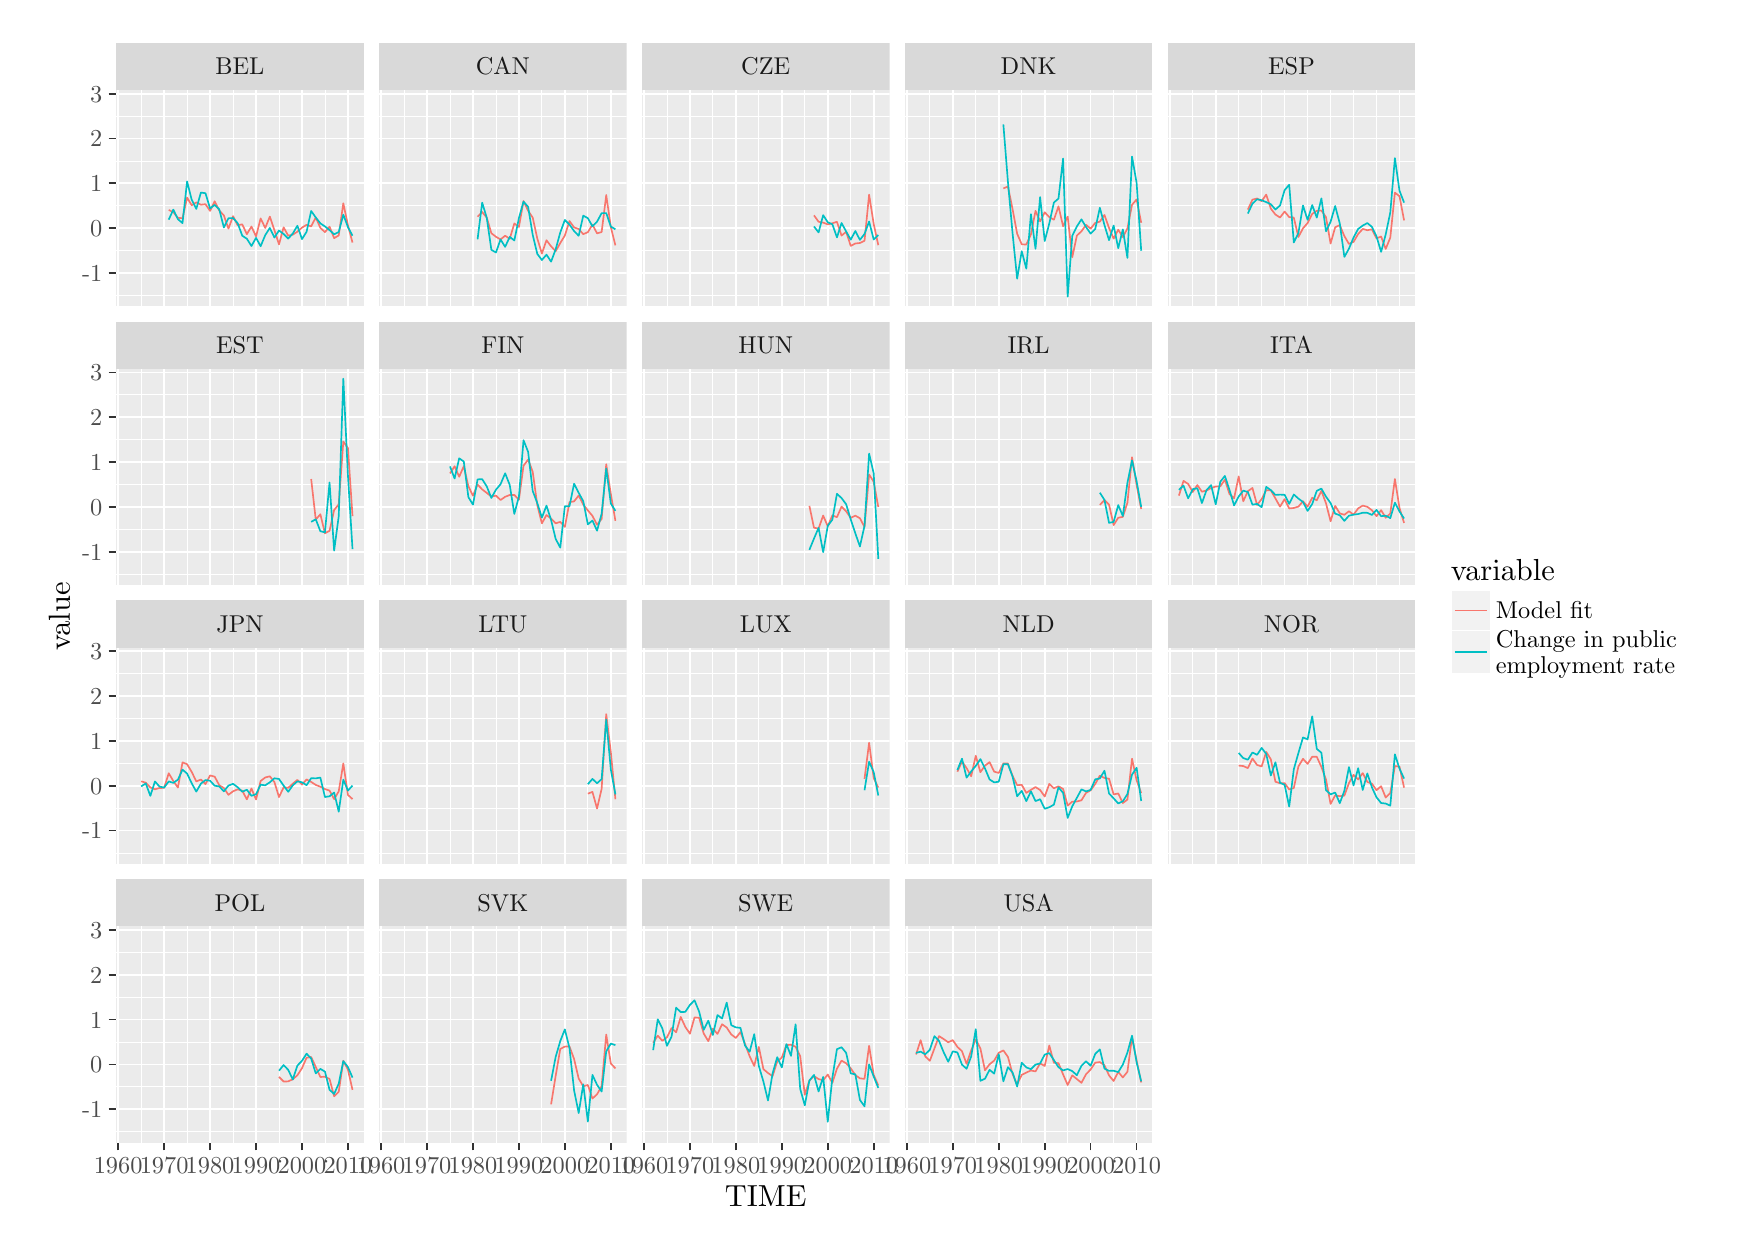
\begin{tikzpicture}[x=1pt,y=1pt]
\definecolor{fillColor}{RGB}{255,255,255}
\path[use as bounding box,fill=fillColor,fill opacity=0.00] (0,0) rectangle (614.29,433.62);
\begin{scope}
\path[clip] (  0.00,  0.00) rectangle (614.29,433.62);
\definecolor{drawColor}{RGB}{255,255,255}
\definecolor{fillColor}{RGB}{255,255,255}

\path[draw=drawColor,line width= 0.6pt,line join=round,line cap=round,fill=fillColor] (  0.00,  0.00) rectangle (614.29,433.62);
\end{scope}
\begin{scope}
\path[clip] ( 31.96,332.89) rectangle (121.45,411.06);
\definecolor{fillColor}{gray}{0.92}

\path[fill=fillColor] ( 31.96,332.89) rectangle (121.45,411.06);
\definecolor{drawColor}{RGB}{255,255,255}

\path[draw=drawColor,line width= 0.3pt,line join=round] ( 31.96,336.87) --
	(121.45,336.87);

\path[draw=drawColor,line width= 0.3pt,line join=round] ( 31.96,353.07) --
	(121.45,353.07);

\path[draw=drawColor,line width= 0.3pt,line join=round] ( 31.96,369.27) --
	(121.45,369.27);

\path[draw=drawColor,line width= 0.3pt,line join=round] ( 31.96,385.46) --
	(121.45,385.46);

\path[draw=drawColor,line width= 0.3pt,line join=round] ( 31.96,401.66) --
	(121.45,401.66);

\path[draw=drawColor,line width= 0.3pt,line join=round] ( 41.01,332.89) --
	( 41.01,411.06);

\path[draw=drawColor,line width= 0.3pt,line join=round] ( 57.61,332.89) --
	( 57.61,411.06);

\path[draw=drawColor,line width= 0.3pt,line join=round] ( 74.21,332.89) --
	( 74.21,411.06);

\path[draw=drawColor,line width= 0.3pt,line join=round] ( 90.82,332.89) --
	( 90.82,411.06);

\path[draw=drawColor,line width= 0.3pt,line join=round] (107.42,332.89) --
	(107.42,411.06);

\path[draw=drawColor,line width= 0.6pt,line join=round] ( 31.96,344.97) --
	(121.45,344.97);

\path[draw=drawColor,line width= 0.6pt,line join=round] ( 31.96,361.17) --
	(121.45,361.17);

\path[draw=drawColor,line width= 0.6pt,line join=round] ( 31.96,377.37) --
	(121.45,377.37);

\path[draw=drawColor,line width= 0.6pt,line join=round] ( 31.96,393.56) --
	(121.45,393.56);

\path[draw=drawColor,line width= 0.6pt,line join=round] ( 31.96,409.76) --
	(121.45,409.76);

\path[draw=drawColor,line width= 0.6pt,line join=round] ( 32.70,332.89) --
	( 32.70,411.06);

\path[draw=drawColor,line width= 0.6pt,line join=round] ( 49.31,332.89) --
	( 49.31,411.06);

\path[draw=drawColor,line width= 0.6pt,line join=round] ( 65.91,332.89) --
	( 65.91,411.06);

\path[draw=drawColor,line width= 0.6pt,line join=round] ( 82.52,332.89) --
	( 82.52,411.06);

\path[draw=drawColor,line width= 0.6pt,line join=round] ( 99.12,332.89) --
	( 99.12,411.06);

\path[draw=drawColor,line width= 0.6pt,line join=round] (115.72,332.89) --
	(115.72,411.06);
\definecolor{drawColor}{RGB}{248,118,109}

\path[draw=drawColor,line width= 0.6pt,line join=round] ( 50.97,367.76) --
	( 52.63,366.93) --
	( 54.29,364.90) --
	( 55.95,364.75) --
	( 57.61,372.22) --
	( 59.27,369.46) --
	( 60.93,370.48) --
	( 62.59,369.64) --
	( 64.25,369.84) --
	( 65.91,367.41) --
	( 67.57,370.90) --
	( 69.23,367.54) --
	( 70.89,365.77) --
	( 72.55,361.00) --
	( 74.21,365.50) --
	( 75.87,362.24) --
	( 77.54,362.54) --
	( 79.20,359.00) --
	( 80.86,361.75) --
	( 82.52,358.18) --
	( 84.18,364.70) --
	( 85.84,361.24) --
	( 87.50,365.35) --
	( 89.16,360.46) --
	( 90.82,355.31) --
	( 92.48,361.47) --
	( 94.14,358.46) --
	( 95.80,358.81) --
	( 97.46,359.90) --
	( 99.12,361.37) --
	(100.78,362.36) --
	(102.44,361.81) --
	(104.10,365.04) --
	(105.76,361.27) --
	(107.42,359.74) --
	(109.08,361.70) --
	(110.74,357.55) --
	(112.40,358.55) --
	(114.06,370.15) --
	(115.72,362.21) --
	(117.38,355.97);
\definecolor{drawColor}{RGB}{0,191,196}

\path[draw=drawColor,line width= 0.6pt,line join=round] ( 50.97,364.25) --
	( 52.63,367.86) --
	( 54.29,364.41) --
	( 55.95,363.00) --
	( 57.61,378.04) --
	( 59.27,371.44) --
	( 60.93,368.11) --
	( 62.59,374.04) --
	( 64.25,373.79) --
	( 65.91,368.29) --
	( 67.57,369.58) --
	( 69.23,367.94) --
	( 70.89,361.43) --
	( 72.55,364.76) --
	( 74.21,364.82) --
	( 75.87,362.99) --
	( 77.54,358.44) --
	( 79.20,357.35) --
	( 80.86,354.72) --
	( 82.52,357.68) --
	( 84.18,354.64) --
	( 85.84,358.64) --
	( 87.50,361.25) --
	( 89.16,357.78) --
	( 90.82,360.31) --
	( 92.48,359.08) --
	( 94.14,357.39) --
	( 95.80,359.23) --
	( 97.46,362.05) --
	( 99.12,357.21) --
	(100.78,359.86) --
	(102.44,367.38) --
	(104.10,365.03) --
	(105.76,362.91) --
	(107.42,361.81) --
	(109.08,360.45) --
	(110.74,358.96) --
	(112.40,359.79) --
	(114.06,366.05) --
	(115.72,361.56) --
	(117.38,358.45);
\end{scope}
\begin{scope}
\path[clip] (126.95,332.89) rectangle (216.45,411.06);
\definecolor{fillColor}{gray}{0.92}

\path[fill=fillColor] (126.95,332.89) rectangle (216.45,411.06);
\definecolor{drawColor}{RGB}{255,255,255}

\path[draw=drawColor,line width= 0.3pt,line join=round] (126.95,336.87) --
	(216.45,336.87);

\path[draw=drawColor,line width= 0.3pt,line join=round] (126.95,353.07) --
	(216.45,353.07);

\path[draw=drawColor,line width= 0.3pt,line join=round] (126.95,369.27) --
	(216.45,369.27);

\path[draw=drawColor,line width= 0.3pt,line join=round] (126.95,385.46) --
	(216.45,385.46);

\path[draw=drawColor,line width= 0.3pt,line join=round] (126.95,401.66) --
	(216.45,401.66);

\path[draw=drawColor,line width= 0.3pt,line join=round] (136.00,332.89) --
	(136.00,411.06);

\path[draw=drawColor,line width= 0.3pt,line join=round] (152.61,332.89) --
	(152.61,411.06);

\path[draw=drawColor,line width= 0.3pt,line join=round] (169.21,332.89) --
	(169.21,411.06);

\path[draw=drawColor,line width= 0.3pt,line join=round] (185.81,332.89) --
	(185.81,411.06);

\path[draw=drawColor,line width= 0.3pt,line join=round] (202.42,332.89) --
	(202.42,411.06);

\path[draw=drawColor,line width= 0.6pt,line join=round] (126.95,344.97) --
	(216.45,344.97);

\path[draw=drawColor,line width= 0.6pt,line join=round] (126.95,361.17) --
	(216.45,361.17);

\path[draw=drawColor,line width= 0.6pt,line join=round] (126.95,377.37) --
	(216.45,377.37);

\path[draw=drawColor,line width= 0.6pt,line join=round] (126.95,393.56) --
	(216.45,393.56);

\path[draw=drawColor,line width= 0.6pt,line join=round] (126.95,409.76) --
	(216.45,409.76);

\path[draw=drawColor,line width= 0.6pt,line join=round] (127.70,332.89) --
	(127.70,411.06);

\path[draw=drawColor,line width= 0.6pt,line join=round] (144.30,332.89) --
	(144.30,411.06);

\path[draw=drawColor,line width= 0.6pt,line join=round] (160.91,332.89) --
	(160.91,411.06);

\path[draw=drawColor,line width= 0.6pt,line join=round] (177.51,332.89) --
	(177.51,411.06);

\path[draw=drawColor,line width= 0.6pt,line join=round] (194.11,332.89) --
	(194.11,411.06);

\path[draw=drawColor,line width= 0.6pt,line join=round] (210.72,332.89) --
	(210.72,411.06);
\definecolor{drawColor}{RGB}{248,118,109}

\path[draw=drawColor,line width= 0.6pt,line join=round] (162.57,365.34) --
	(164.23,366.99) --
	(165.89,364.97) --
	(167.55,359.34) --
	(169.21,358.06) --
	(170.87,357.10) --
	(172.53,358.43) --
	(174.19,357.31) --
	(175.85,362.87) --
	(177.51,361.60) --
	(179.17,370.98) --
	(180.83,367.45) --
	(182.49,365.00) --
	(184.15,357.44) --
	(185.81,351.99) --
	(187.47,356.80) --
	(189.13,354.61) --
	(190.79,352.83) --
	(192.45,355.80) --
	(194.11,358.52) --
	(195.78,363.74) --
	(197.44,361.45) --
	(199.10,360.85) --
	(200.76,359.00) --
	(202.42,359.72) --
	(204.08,362.46) --
	(205.74,359.29) --
	(207.40,359.76) --
	(209.06,373.13) --
	(210.72,361.55) --
	(212.38,354.95);
\definecolor{drawColor}{RGB}{0,191,196}

\path[draw=drawColor,line width= 0.6pt,line join=round] (162.57,357.14) --
	(164.23,370.41) --
	(165.89,364.91) --
	(167.55,353.34) --
	(169.21,352.38) --
	(170.87,357.09) --
	(172.53,354.41) --
	(174.19,358.01) --
	(175.85,356.72) --
	(177.51,364.83) --
	(179.17,370.74) --
	(180.83,368.90) --
	(182.49,358.76) --
	(184.15,351.88) --
	(185.81,349.66) --
	(187.47,351.58) --
	(189.13,349.07) --
	(190.79,353.53) --
	(192.45,359.60) --
	(194.11,364.14) --
	(195.78,362.46) --
	(197.44,360.14) --
	(199.10,358.41) --
	(200.76,365.69) --
	(202.42,364.78) --
	(204.08,361.83) --
	(205.74,363.51) --
	(207.40,366.60) --
	(209.06,366.61) --
	(210.72,361.76) --
	(212.38,360.74);
\end{scope}
\begin{scope}
\path[clip] (221.95,332.89) rectangle (311.44,411.06);
\definecolor{fillColor}{gray}{0.92}

\path[fill=fillColor] (221.95,332.89) rectangle (311.44,411.06);
\definecolor{drawColor}{RGB}{255,255,255}

\path[draw=drawColor,line width= 0.3pt,line join=round] (221.95,336.87) --
	(311.44,336.87);

\path[draw=drawColor,line width= 0.3pt,line join=round] (221.95,353.07) --
	(311.44,353.07);

\path[draw=drawColor,line width= 0.3pt,line join=round] (221.95,369.27) --
	(311.44,369.27);

\path[draw=drawColor,line width= 0.3pt,line join=round] (221.95,385.46) --
	(311.44,385.46);

\path[draw=drawColor,line width= 0.3pt,line join=round] (221.95,401.66) --
	(311.44,401.66);

\path[draw=drawColor,line width= 0.3pt,line join=round] (231.00,332.89) --
	(231.00,411.06);

\path[draw=drawColor,line width= 0.3pt,line join=round] (247.60,332.89) --
	(247.60,411.06);

\path[draw=drawColor,line width= 0.3pt,line join=round] (264.20,332.89) --
	(264.20,411.06);

\path[draw=drawColor,line width= 0.3pt,line join=round] (280.81,332.89) --
	(280.81,411.06);

\path[draw=drawColor,line width= 0.3pt,line join=round] (297.41,332.89) --
	(297.41,411.06);

\path[draw=drawColor,line width= 0.6pt,line join=round] (221.95,344.97) --
	(311.44,344.97);

\path[draw=drawColor,line width= 0.6pt,line join=round] (221.95,361.17) --
	(311.44,361.17);

\path[draw=drawColor,line width= 0.6pt,line join=round] (221.95,377.37) --
	(311.44,377.37);

\path[draw=drawColor,line width= 0.6pt,line join=round] (221.95,393.56) --
	(311.44,393.56);

\path[draw=drawColor,line width= 0.6pt,line join=round] (221.95,409.76) --
	(311.44,409.76);

\path[draw=drawColor,line width= 0.6pt,line join=round] (222.69,332.89) --
	(222.69,411.06);

\path[draw=drawColor,line width= 0.6pt,line join=round] (239.30,332.89) --
	(239.30,411.06);

\path[draw=drawColor,line width= 0.6pt,line join=round] (255.90,332.89) --
	(255.90,411.06);

\path[draw=drawColor,line width= 0.6pt,line join=round] (272.51,332.89) --
	(272.51,411.06);

\path[draw=drawColor,line width= 0.6pt,line join=round] (289.11,332.89) --
	(289.11,411.06);

\path[draw=drawColor,line width= 0.6pt,line join=round] (305.71,332.89) --
	(305.71,411.06);
\definecolor{drawColor}{RGB}{248,118,109}

\path[draw=drawColor,line width= 0.6pt,line join=round] (284.13,365.80) --
	(285.79,363.48) --
	(287.45,363.18) --
	(289.11,362.54) --
	(290.77,362.92) --
	(292.43,363.47) --
	(294.09,358.49) --
	(295.75,359.84) --
	(297.41,354.76) --
	(299.07,355.63) --
	(300.73,355.81) --
	(302.39,356.62) --
	(304.05,373.27) --
	(305.71,362.68) --
	(307.37,355.03);
\definecolor{drawColor}{RGB}{0,191,196}

\path[draw=drawColor,line width= 0.6pt,line join=round] (284.13,361.78) --
	(285.79,359.63) --
	(287.45,365.87) --
	(289.11,363.29) --
	(290.77,362.59) --
	(292.43,357.83) --
	(294.09,363.03) --
	(295.75,359.98) --
	(297.41,357.01) --
	(299.07,360.14) --
	(300.73,356.93) --
	(302.39,359.09) --
	(304.05,363.57) --
	(305.71,357.07) --
	(307.37,358.68);
\end{scope}
\begin{scope}
\path[clip] (316.94,332.89) rectangle (406.44,411.06);
\definecolor{fillColor}{gray}{0.92}

\path[fill=fillColor] (316.94,332.89) rectangle (406.44,411.06);
\definecolor{drawColor}{RGB}{255,255,255}

\path[draw=drawColor,line width= 0.3pt,line join=round] (316.94,336.87) --
	(406.44,336.87);

\path[draw=drawColor,line width= 0.3pt,line join=round] (316.94,353.07) --
	(406.44,353.07);

\path[draw=drawColor,line width= 0.3pt,line join=round] (316.94,369.27) --
	(406.44,369.27);

\path[draw=drawColor,line width= 0.3pt,line join=round] (316.94,385.46) --
	(406.44,385.46);

\path[draw=drawColor,line width= 0.3pt,line join=round] (316.94,401.66) --
	(406.44,401.66);

\path[draw=drawColor,line width= 0.3pt,line join=round] (325.99,332.89) --
	(325.99,411.06);

\path[draw=drawColor,line width= 0.3pt,line join=round] (342.59,332.89) --
	(342.59,411.06);

\path[draw=drawColor,line width= 0.3pt,line join=round] (359.20,332.89) --
	(359.20,411.06);

\path[draw=drawColor,line width= 0.3pt,line join=round] (375.80,332.89) --
	(375.80,411.06);

\path[draw=drawColor,line width= 0.3pt,line join=round] (392.41,332.89) --
	(392.41,411.06);

\path[draw=drawColor,line width= 0.6pt,line join=round] (316.94,344.97) --
	(406.44,344.97);

\path[draw=drawColor,line width= 0.6pt,line join=round] (316.94,361.17) --
	(406.44,361.17);

\path[draw=drawColor,line width= 0.6pt,line join=round] (316.94,377.37) --
	(406.44,377.37);

\path[draw=drawColor,line width= 0.6pt,line join=round] (316.94,393.56) --
	(406.44,393.56);

\path[draw=drawColor,line width= 0.6pt,line join=round] (316.94,409.76) --
	(406.44,409.76);

\path[draw=drawColor,line width= 0.6pt,line join=round] (317.69,332.89) --
	(317.69,411.06);

\path[draw=drawColor,line width= 0.6pt,line join=round] (334.29,332.89) --
	(334.29,411.06);

\path[draw=drawColor,line width= 0.6pt,line join=round] (350.90,332.89) --
	(350.90,411.06);

\path[draw=drawColor,line width= 0.6pt,line join=round] (367.50,332.89) --
	(367.50,411.06);

\path[draw=drawColor,line width= 0.6pt,line join=round] (384.10,332.89) --
	(384.10,411.06);

\path[draw=drawColor,line width= 0.6pt,line join=round] (400.71,332.89) --
	(400.71,411.06);
\definecolor{drawColor}{RGB}{248,118,109}

\path[draw=drawColor,line width= 0.6pt,line join=round] (352.56,375.52) --
	(354.22,376.24) --
	(355.88,368.09) --
	(357.54,359.17) --
	(359.20,355.33) --
	(360.86,355.26) --
	(362.52,358.90) --
	(364.18,367.42) --
	(365.84,363.62) --
	(367.50,366.90) --
	(369.16,365.16) --
	(370.82,364.22) --
	(372.48,369.04) --
	(374.14,361.87) --
	(375.80,365.35) --
	(377.46,350.65) --
	(379.12,358.48) --
	(380.78,360.04) --
	(382.44,362.37) --
	(384.10,361.00) --
	(385.76,363.07) --
	(387.43,363.53) --
	(389.09,365.94) --
	(390.75,361.23) --
	(392.41,357.38) --
	(394.07,360.62) --
	(395.73,357.92) --
	(397.39,361.06) --
	(399.05,369.61) --
	(400.71,371.55) --
	(402.37,363.12);
\definecolor{drawColor}{RGB}{0,191,196}

\path[draw=drawColor,line width= 0.6pt,line join=round] (352.56,398.68) --
	(354.22,377.83) --
	(355.88,359.41) --
	(357.54,342.91) --
	(359.20,352.83) --
	(360.86,346.54) --
	(362.52,366.21) --
	(364.18,353.71) --
	(365.84,372.41) --
	(367.50,356.51) --
	(369.16,362.88) --
	(370.82,370.43) --
	(372.48,371.86) --
	(374.14,386.33) --
	(375.80,336.44) --
	(377.46,358.39) --
	(379.12,361.79) --
	(380.78,364.36) --
	(382.44,361.57) --
	(384.10,359.18) --
	(385.76,360.87) --
	(387.43,368.53) --
	(389.09,362.29) --
	(390.75,356.83) --
	(392.41,362.11) --
	(394.07,353.94) --
	(395.73,360.73) --
	(397.39,350.41) --
	(399.05,387.03) --
	(400.71,377.55) --
	(402.37,353.01);
\end{scope}
\begin{scope}
\path[clip] (411.94,332.89) rectangle (501.43,411.06);
\definecolor{fillColor}{gray}{0.92}

\path[fill=fillColor] (411.94,332.89) rectangle (501.43,411.06);
\definecolor{drawColor}{RGB}{255,255,255}

\path[draw=drawColor,line width= 0.3pt,line join=round] (411.94,336.87) --
	(501.43,336.87);

\path[draw=drawColor,line width= 0.3pt,line join=round] (411.94,353.07) --
	(501.43,353.07);

\path[draw=drawColor,line width= 0.3pt,line join=round] (411.94,369.27) --
	(501.43,369.27);

\path[draw=drawColor,line width= 0.3pt,line join=round] (411.94,385.46) --
	(501.43,385.46);

\path[draw=drawColor,line width= 0.3pt,line join=round] (411.94,401.66) --
	(501.43,401.66);

\path[draw=drawColor,line width= 0.3pt,line join=round] (420.99,332.89) --
	(420.99,411.06);

\path[draw=drawColor,line width= 0.3pt,line join=round] (437.59,332.89) --
	(437.59,411.06);

\path[draw=drawColor,line width= 0.3pt,line join=round] (454.19,332.89) --
	(454.19,411.06);

\path[draw=drawColor,line width= 0.3pt,line join=round] (470.80,332.89) --
	(470.80,411.06);

\path[draw=drawColor,line width= 0.3pt,line join=round] (487.40,332.89) --
	(487.40,411.06);

\path[draw=drawColor,line width= 0.6pt,line join=round] (411.94,344.97) --
	(501.43,344.97);

\path[draw=drawColor,line width= 0.6pt,line join=round] (411.94,361.17) --
	(501.43,361.17);

\path[draw=drawColor,line width= 0.6pt,line join=round] (411.94,377.37) --
	(501.43,377.37);

\path[draw=drawColor,line width= 0.6pt,line join=round] (411.94,393.56) --
	(501.43,393.56);

\path[draw=drawColor,line width= 0.6pt,line join=round] (411.94,409.76) --
	(501.43,409.76);

\path[draw=drawColor,line width= 0.6pt,line join=round] (412.68,332.89) --
	(412.68,411.06);

\path[draw=drawColor,line width= 0.6pt,line join=round] (429.29,332.89) --
	(429.29,411.06);

\path[draw=drawColor,line width= 0.6pt,line join=round] (445.89,332.89) --
	(445.89,411.06);

\path[draw=drawColor,line width= 0.6pt,line join=round] (462.50,332.89) --
	(462.50,411.06);

\path[draw=drawColor,line width= 0.6pt,line join=round] (479.10,332.89) --
	(479.10,411.06);

\path[draw=drawColor,line width= 0.6pt,line join=round] (495.70,332.89) --
	(495.70,411.06);
\definecolor{drawColor}{RGB}{248,118,109}

\path[draw=drawColor,line width= 0.6pt,line join=round] (440.91,367.87) --
	(442.57,371.48) --
	(444.23,371.89) --
	(445.89,370.93) --
	(447.55,373.30) --
	(449.21,368.22) --
	(450.87,366.09) --
	(452.53,365.01) --
	(454.19,367.17) --
	(455.85,365.16) --
	(457.51,364.98) --
	(459.17,357.98) --
	(460.83,361.10) --
	(462.50,363.03) --
	(464.16,366.31) --
	(465.82,367.42) --
	(467.48,367.55) --
	(469.14,365.14) --
	(470.80,355.61) --
	(472.46,361.48) --
	(474.12,362.28) --
	(475.78,358.30) --
	(477.44,355.47) --
	(479.10,356.22) --
	(480.76,359.05) --
	(482.42,360.89) --
	(484.08,360.43) --
	(485.74,360.73) --
	(487.40,357.47) --
	(489.06,358.15) --
	(490.72,353.66) --
	(492.38,357.77) --
	(494.04,374.01) --
	(495.70,372.70) --
	(497.36,363.98);
\definecolor{drawColor}{RGB}{0,191,196}

\path[draw=drawColor,line width= 0.6pt,line join=round] (440.91,366.45) --
	(442.57,370.03) --
	(444.23,371.60) --
	(445.89,371.26) --
	(447.55,370.58) --
	(449.21,369.82) --
	(450.87,367.90) --
	(452.53,369.36) --
	(454.19,374.91) --
	(455.85,376.85) --
	(457.51,356.01) --
	(459.17,359.40) --
	(460.83,369.35) --
	(462.50,364.15) --
	(464.16,369.51) --
	(465.82,364.98) --
	(467.48,371.94) --
	(469.14,360.04) --
	(470.80,363.47) --
	(472.46,369.17) --
	(474.12,362.89) --
	(475.78,350.78) --
	(477.44,353.77) --
	(479.10,357.78) --
	(480.76,360.88) --
	(482.42,362.10) --
	(484.08,363.01) --
	(485.74,361.63) --
	(487.40,358.18) --
	(489.06,352.59) --
	(490.72,358.92) --
	(492.38,366.83) --
	(494.04,386.49) --
	(495.70,374.68) --
	(497.36,370.41);
\end{scope}
\begin{scope}
\path[clip] ( 31.96,232.15) rectangle (121.45,310.33);
\definecolor{fillColor}{gray}{0.92}

\path[fill=fillColor] ( 31.96,232.15) rectangle (121.45,310.33);
\definecolor{drawColor}{RGB}{255,255,255}

\path[draw=drawColor,line width= 0.3pt,line join=round] ( 31.96,236.14) --
	(121.45,236.14);

\path[draw=drawColor,line width= 0.3pt,line join=round] ( 31.96,252.34) --
	(121.45,252.34);

\path[draw=drawColor,line width= 0.3pt,line join=round] ( 31.96,268.53) --
	(121.45,268.53);

\path[draw=drawColor,line width= 0.3pt,line join=round] ( 31.96,284.73) --
	(121.45,284.73);

\path[draw=drawColor,line width= 0.3pt,line join=round] ( 31.96,300.93) --
	(121.45,300.93);

\path[draw=drawColor,line width= 0.3pt,line join=round] ( 41.01,232.15) --
	( 41.01,310.33);

\path[draw=drawColor,line width= 0.3pt,line join=round] ( 57.61,232.15) --
	( 57.61,310.33);

\path[draw=drawColor,line width= 0.3pt,line join=round] ( 74.21,232.15) --
	( 74.21,310.33);

\path[draw=drawColor,line width= 0.3pt,line join=round] ( 90.82,232.15) --
	( 90.82,310.33);

\path[draw=drawColor,line width= 0.3pt,line join=round] (107.42,232.15) --
	(107.42,310.33);

\path[draw=drawColor,line width= 0.6pt,line join=round] ( 31.96,244.24) --
	(121.45,244.24);

\path[draw=drawColor,line width= 0.6pt,line join=round] ( 31.96,260.44) --
	(121.45,260.44);

\path[draw=drawColor,line width= 0.6pt,line join=round] ( 31.96,276.63) --
	(121.45,276.63);

\path[draw=drawColor,line width= 0.6pt,line join=round] ( 31.96,292.83) --
	(121.45,292.83);

\path[draw=drawColor,line width= 0.6pt,line join=round] ( 31.96,309.03) --
	(121.45,309.03);

\path[draw=drawColor,line width= 0.6pt,line join=round] ( 32.70,232.15) --
	( 32.70,310.33);

\path[draw=drawColor,line width= 0.6pt,line join=round] ( 49.31,232.15) --
	( 49.31,310.33);

\path[draw=drawColor,line width= 0.6pt,line join=round] ( 65.91,232.15) --
	( 65.91,310.33);

\path[draw=drawColor,line width= 0.6pt,line join=round] ( 82.52,232.15) --
	( 82.52,310.33);

\path[draw=drawColor,line width= 0.6pt,line join=round] ( 99.12,232.15) --
	( 99.12,310.33);

\path[draw=drawColor,line width= 0.6pt,line join=round] (115.72,232.15) --
	(115.72,310.33);
\definecolor{drawColor}{RGB}{248,118,109}

\path[draw=drawColor,line width= 0.6pt,line join=round] (102.44,270.52) --
	(104.10,255.86) --
	(105.76,257.79) --
	(107.42,250.92) --
	(109.08,251.81) --
	(110.74,259.32) --
	(112.40,261.37) --
	(114.06,284.07) --
	(115.72,281.74) --
	(117.38,257.12);
\definecolor{drawColor}{RGB}{0,191,196}

\path[draw=drawColor,line width= 0.6pt,line join=round] (102.44,255.04) --
	(104.10,255.97) --
	(105.76,251.67) --
	(107.42,251.25) --
	(109.08,269.27) --
	(110.74,244.68) --
	(112.40,257.10) --
	(114.06,306.77) --
	(115.72,271.92) --
	(117.38,245.17);
\end{scope}
\begin{scope}
\path[clip] (126.95,232.15) rectangle (216.45,310.33);
\definecolor{fillColor}{gray}{0.92}

\path[fill=fillColor] (126.95,232.15) rectangle (216.45,310.33);
\definecolor{drawColor}{RGB}{255,255,255}

\path[draw=drawColor,line width= 0.3pt,line join=round] (126.95,236.14) --
	(216.45,236.14);

\path[draw=drawColor,line width= 0.3pt,line join=round] (126.95,252.34) --
	(216.45,252.34);

\path[draw=drawColor,line width= 0.3pt,line join=round] (126.95,268.53) --
	(216.45,268.53);

\path[draw=drawColor,line width= 0.3pt,line join=round] (126.95,284.73) --
	(216.45,284.73);

\path[draw=drawColor,line width= 0.3pt,line join=round] (126.95,300.93) --
	(216.45,300.93);

\path[draw=drawColor,line width= 0.3pt,line join=round] (136.00,232.15) --
	(136.00,310.33);

\path[draw=drawColor,line width= 0.3pt,line join=round] (152.61,232.15) --
	(152.61,310.33);

\path[draw=drawColor,line width= 0.3pt,line join=round] (169.21,232.15) --
	(169.21,310.33);

\path[draw=drawColor,line width= 0.3pt,line join=round] (185.81,232.15) --
	(185.81,310.33);

\path[draw=drawColor,line width= 0.3pt,line join=round] (202.42,232.15) --
	(202.42,310.33);

\path[draw=drawColor,line width= 0.6pt,line join=round] (126.95,244.24) --
	(216.45,244.24);

\path[draw=drawColor,line width= 0.6pt,line join=round] (126.95,260.44) --
	(216.45,260.44);

\path[draw=drawColor,line width= 0.6pt,line join=round] (126.95,276.63) --
	(216.45,276.63);

\path[draw=drawColor,line width= 0.6pt,line join=round] (126.95,292.83) --
	(216.45,292.83);

\path[draw=drawColor,line width= 0.6pt,line join=round] (126.95,309.03) --
	(216.45,309.03);

\path[draw=drawColor,line width= 0.6pt,line join=round] (127.70,232.15) --
	(127.70,310.33);

\path[draw=drawColor,line width= 0.6pt,line join=round] (144.30,232.15) --
	(144.30,310.33);

\path[draw=drawColor,line width= 0.6pt,line join=round] (160.91,232.15) --
	(160.91,310.33);

\path[draw=drawColor,line width= 0.6pt,line join=round] (177.51,232.15) --
	(177.51,310.33);

\path[draw=drawColor,line width= 0.6pt,line join=round] (194.11,232.15) --
	(194.11,310.33);

\path[draw=drawColor,line width= 0.6pt,line join=round] (210.72,232.15) --
	(210.72,310.33);
\definecolor{drawColor}{RGB}{248,118,109}

\path[draw=drawColor,line width= 0.6pt,line join=round] (152.61,272.55) --
	(154.27,275.13) --
	(155.93,271.34) --
	(157.59,275.16) --
	(159.25,267.89) --
	(160.91,264.49) --
	(162.57,268.52) --
	(164.23,266.78) --
	(165.89,265.50) --
	(167.55,264.19) --
	(169.21,264.52) --
	(170.87,262.93) --
	(172.53,264.10) --
	(174.19,264.75) --
	(175.85,264.77) --
	(177.51,263.04) --
	(179.17,275.31) --
	(180.83,277.56) --
	(182.49,273.13) --
	(184.15,261.10) --
	(185.81,254.49) --
	(187.47,257.51) --
	(189.13,256.26) --
	(190.79,254.51) --
	(192.45,255.03) --
	(194.11,253.21) --
	(195.78,262.16) --
	(197.44,262.45) --
	(199.10,264.56) --
	(200.76,261.28) --
	(202.42,259.18) --
	(204.08,257.20) --
	(205.74,253.99) --
	(207.40,256.10) --
	(209.06,275.85) --
	(210.72,265.13) --
	(212.38,255.42);
\definecolor{drawColor}{RGB}{0,191,196}

\path[draw=drawColor,line width= 0.6pt,line join=round] (152.61,275.05) --
	(154.27,270.72) --
	(155.93,278.01) --
	(157.59,276.84) --
	(159.25,263.97) --
	(160.91,261.25) --
	(162.57,270.39) --
	(164.23,270.48) --
	(165.89,267.85) --
	(167.55,263.68) --
	(169.21,266.66) --
	(170.87,268.65) --
	(172.53,272.59) --
	(174.19,268.39) --
	(175.85,257.91) --
	(177.51,264.19) --
	(179.17,284.54) --
	(180.83,280.35) --
	(182.49,266.20) --
	(184.15,261.84) --
	(185.81,256.57) --
	(187.47,260.91) --
	(189.13,255.73) --
	(190.79,248.88) --
	(192.45,245.73) --
	(194.11,260.71) --
	(195.78,260.70) --
	(197.44,268.82) --
	(199.10,265.56) --
	(200.76,262.49) --
	(202.42,254.12) --
	(204.08,255.52) --
	(205.74,251.84) --
	(207.40,257.99) --
	(209.06,274.30) --
	(210.72,261.65) --
	(212.38,259.03);
\end{scope}
\begin{scope}
\path[clip] (221.95,232.15) rectangle (311.44,310.33);
\definecolor{fillColor}{gray}{0.92}

\path[fill=fillColor] (221.95,232.15) rectangle (311.44,310.33);
\definecolor{drawColor}{RGB}{255,255,255}

\path[draw=drawColor,line width= 0.3pt,line join=round] (221.95,236.14) --
	(311.44,236.14);

\path[draw=drawColor,line width= 0.3pt,line join=round] (221.95,252.34) --
	(311.44,252.34);

\path[draw=drawColor,line width= 0.3pt,line join=round] (221.95,268.53) --
	(311.44,268.53);

\path[draw=drawColor,line width= 0.3pt,line join=round] (221.95,284.73) --
	(311.44,284.73);

\path[draw=drawColor,line width= 0.3pt,line join=round] (221.95,300.93) --
	(311.44,300.93);

\path[draw=drawColor,line width= 0.3pt,line join=round] (231.00,232.15) --
	(231.00,310.33);

\path[draw=drawColor,line width= 0.3pt,line join=round] (247.60,232.15) --
	(247.60,310.33);

\path[draw=drawColor,line width= 0.3pt,line join=round] (264.20,232.15) --
	(264.20,310.33);

\path[draw=drawColor,line width= 0.3pt,line join=round] (280.81,232.15) --
	(280.81,310.33);

\path[draw=drawColor,line width= 0.3pt,line join=round] (297.41,232.15) --
	(297.41,310.33);

\path[draw=drawColor,line width= 0.6pt,line join=round] (221.95,244.24) --
	(311.44,244.24);

\path[draw=drawColor,line width= 0.6pt,line join=round] (221.95,260.44) --
	(311.44,260.44);

\path[draw=drawColor,line width= 0.6pt,line join=round] (221.95,276.63) --
	(311.44,276.63);

\path[draw=drawColor,line width= 0.6pt,line join=round] (221.95,292.83) --
	(311.44,292.83);

\path[draw=drawColor,line width= 0.6pt,line join=round] (221.95,309.03) --
	(311.44,309.03);

\path[draw=drawColor,line width= 0.6pt,line join=round] (222.69,232.15) --
	(222.69,310.33);

\path[draw=drawColor,line width= 0.6pt,line join=round] (239.30,232.15) --
	(239.30,310.33);

\path[draw=drawColor,line width= 0.6pt,line join=round] (255.90,232.15) --
	(255.90,310.33);

\path[draw=drawColor,line width= 0.6pt,line join=round] (272.51,232.15) --
	(272.51,310.33);

\path[draw=drawColor,line width= 0.6pt,line join=round] (289.11,232.15) --
	(289.11,310.33);

\path[draw=drawColor,line width= 0.6pt,line join=round] (305.71,232.15) --
	(305.71,310.33);
\definecolor{drawColor}{RGB}{248,118,109}

\path[draw=drawColor,line width= 0.6pt,line join=round] (282.47,260.82) --
	(284.13,252.92) --
	(285.79,252.63) --
	(287.45,257.33) --
	(289.11,253.42) --
	(290.77,257.39) --
	(292.43,256.72) --
	(294.09,260.55) --
	(295.75,258.86) --
	(297.41,256.48) --
	(299.07,257.28) --
	(300.73,256.35) --
	(302.39,253.18) --
	(304.05,272.16) --
	(305.71,269.53) --
	(307.37,260.40);
\definecolor{drawColor}{RGB}{0,191,196}

\path[draw=drawColor,line width= 0.6pt,line join=round] (282.47,244.94) --
	(284.13,249.00) --
	(285.79,252.88) --
	(287.45,244.09) --
	(289.11,253.60) --
	(290.77,255.83) --
	(292.43,265.19) --
	(294.09,263.63) --
	(295.75,261.41) --
	(297.41,255.93) --
	(299.07,250.90) --
	(300.73,246.14) --
	(302.39,253.60) --
	(304.05,279.73) --
	(305.71,272.54) --
	(307.37,241.65);
\end{scope}
\begin{scope}
\path[clip] (316.94,232.15) rectangle (406.44,310.33);
\definecolor{fillColor}{gray}{0.92}

\path[fill=fillColor] (316.94,232.15) rectangle (406.44,310.33);
\definecolor{drawColor}{RGB}{255,255,255}

\path[draw=drawColor,line width= 0.3pt,line join=round] (316.94,236.14) --
	(406.44,236.14);

\path[draw=drawColor,line width= 0.3pt,line join=round] (316.94,252.34) --
	(406.44,252.34);

\path[draw=drawColor,line width= 0.3pt,line join=round] (316.94,268.53) --
	(406.44,268.53);

\path[draw=drawColor,line width= 0.3pt,line join=round] (316.94,284.73) --
	(406.44,284.73);

\path[draw=drawColor,line width= 0.3pt,line join=round] (316.94,300.93) --
	(406.44,300.93);

\path[draw=drawColor,line width= 0.3pt,line join=round] (325.99,232.15) --
	(325.99,310.33);

\path[draw=drawColor,line width= 0.3pt,line join=round] (342.59,232.15) --
	(342.59,310.33);

\path[draw=drawColor,line width= 0.3pt,line join=round] (359.20,232.15) --
	(359.20,310.33);

\path[draw=drawColor,line width= 0.3pt,line join=round] (375.80,232.15) --
	(375.80,310.33);

\path[draw=drawColor,line width= 0.3pt,line join=round] (392.41,232.15) --
	(392.41,310.33);

\path[draw=drawColor,line width= 0.6pt,line join=round] (316.94,244.24) --
	(406.44,244.24);

\path[draw=drawColor,line width= 0.6pt,line join=round] (316.94,260.44) --
	(406.44,260.44);

\path[draw=drawColor,line width= 0.6pt,line join=round] (316.94,276.63) --
	(406.44,276.63);

\path[draw=drawColor,line width= 0.6pt,line join=round] (316.94,292.83) --
	(406.44,292.83);

\path[draw=drawColor,line width= 0.6pt,line join=round] (316.94,309.03) --
	(406.44,309.03);

\path[draw=drawColor,line width= 0.6pt,line join=round] (317.69,232.15) --
	(317.69,310.33);

\path[draw=drawColor,line width= 0.6pt,line join=round] (334.29,232.15) --
	(334.29,310.33);

\path[draw=drawColor,line width= 0.6pt,line join=round] (350.90,232.15) --
	(350.90,310.33);

\path[draw=drawColor,line width= 0.6pt,line join=round] (367.50,232.15) --
	(367.50,310.33);

\path[draw=drawColor,line width= 0.6pt,line join=round] (384.10,232.15) --
	(384.10,310.33);

\path[draw=drawColor,line width= 0.6pt,line join=round] (400.71,232.15) --
	(400.71,310.33);
\definecolor{drawColor}{RGB}{248,118,109}

\path[draw=drawColor,line width= 0.6pt,line join=round] (387.43,261.18) --
	(389.09,262.90) --
	(390.75,261.24) --
	(392.41,253.88) --
	(394.07,256.53) --
	(395.73,256.84) --
	(397.39,261.98) --
	(399.05,278.38) --
	(400.71,268.32) --
	(402.37,259.68);
\definecolor{drawColor}{RGB}{0,191,196}

\path[draw=drawColor,line width= 0.6pt,line join=round] (387.43,265.58) --
	(389.09,262.98) --
	(390.75,254.66) --
	(392.41,255.04) --
	(394.07,261.11) --
	(395.73,257.16) --
	(397.39,269.16) --
	(399.05,277.25) --
	(400.71,269.76) --
	(402.37,260.45);
\end{scope}
\begin{scope}
\path[clip] (411.94,232.15) rectangle (501.43,310.33);
\definecolor{fillColor}{gray}{0.92}

\path[fill=fillColor] (411.94,232.15) rectangle (501.43,310.33);
\definecolor{drawColor}{RGB}{255,255,255}

\path[draw=drawColor,line width= 0.3pt,line join=round] (411.94,236.14) --
	(501.43,236.14);

\path[draw=drawColor,line width= 0.3pt,line join=round] (411.94,252.34) --
	(501.43,252.34);

\path[draw=drawColor,line width= 0.3pt,line join=round] (411.94,268.53) --
	(501.43,268.53);

\path[draw=drawColor,line width= 0.3pt,line join=round] (411.94,284.73) --
	(501.43,284.73);

\path[draw=drawColor,line width= 0.3pt,line join=round] (411.94,300.93) --
	(501.43,300.93);

\path[draw=drawColor,line width= 0.3pt,line join=round] (420.99,232.15) --
	(420.99,310.33);

\path[draw=drawColor,line width= 0.3pt,line join=round] (437.59,232.15) --
	(437.59,310.33);

\path[draw=drawColor,line width= 0.3pt,line join=round] (454.19,232.15) --
	(454.19,310.33);

\path[draw=drawColor,line width= 0.3pt,line join=round] (470.80,232.15) --
	(470.80,310.33);

\path[draw=drawColor,line width= 0.3pt,line join=round] (487.40,232.15) --
	(487.40,310.33);

\path[draw=drawColor,line width= 0.6pt,line join=round] (411.94,244.24) --
	(501.43,244.24);

\path[draw=drawColor,line width= 0.6pt,line join=round] (411.94,260.44) --
	(501.43,260.44);

\path[draw=drawColor,line width= 0.6pt,line join=round] (411.94,276.63) --
	(501.43,276.63);

\path[draw=drawColor,line width= 0.6pt,line join=round] (411.94,292.83) --
	(501.43,292.83);

\path[draw=drawColor,line width= 0.6pt,line join=round] (411.94,309.03) --
	(501.43,309.03);

\path[draw=drawColor,line width= 0.6pt,line join=round] (412.68,232.15) --
	(412.68,310.33);

\path[draw=drawColor,line width= 0.6pt,line join=round] (429.29,232.15) --
	(429.29,310.33);

\path[draw=drawColor,line width= 0.6pt,line join=round] (445.89,232.15) --
	(445.89,310.33);

\path[draw=drawColor,line width= 0.6pt,line join=round] (462.50,232.15) --
	(462.50,310.33);

\path[draw=drawColor,line width= 0.6pt,line join=round] (479.10,232.15) --
	(479.10,310.33);

\path[draw=drawColor,line width= 0.6pt,line join=round] (495.70,232.15) --
	(495.70,310.33);
\definecolor{drawColor}{RGB}{248,118,109}

\path[draw=drawColor,line width= 0.6pt,line join=round] (416.00,264.54) --
	(417.66,269.85) --
	(419.33,268.75) --
	(420.99,265.85) --
	(422.65,268.34) --
	(424.31,265.94) --
	(425.97,266.38) --
	(427.63,267.24) --
	(429.29,267.83) --
	(430.95,267.89) --
	(432.61,270.30) --
	(434.27,265.08) --
	(435.93,263.56) --
	(437.59,271.44) --
	(439.25,262.49) --
	(440.91,266.13) --
	(442.57,267.28) --
	(444.23,261.15) --
	(445.89,263.27) --
	(447.55,266.50) --
	(449.21,266.42) --
	(450.87,263.50) --
	(452.53,260.54) --
	(454.19,263.27) --
	(455.85,259.88) --
	(457.51,260.06) --
	(459.17,260.55) --
	(460.83,262.47) --
	(462.50,260.55) --
	(464.16,263.75) --
	(465.82,262.84) --
	(467.48,266.24) --
	(469.14,261.76) --
	(470.80,255.25) --
	(472.46,260.82) --
	(474.12,258.11) --
	(475.78,257.60) --
	(477.44,258.88) --
	(479.10,257.65) --
	(480.76,259.90) --
	(482.42,260.93) --
	(484.08,260.47) --
	(485.74,259.23) --
	(487.40,257.10) --
	(489.06,259.26) --
	(490.72,256.53) --
	(492.38,258.06) --
	(494.04,270.53) --
	(495.70,260.06) --
	(497.36,254.65);
\definecolor{drawColor}{RGB}{0,191,196}

\path[draw=drawColor,line width= 0.6pt,line join=round] (416.00,266.64) --
	(417.66,268.13) --
	(419.33,263.54) --
	(420.99,266.84) --
	(422.65,267.21) --
	(424.31,261.83) --
	(425.97,266.51) --
	(427.63,268.32) --
	(429.29,261.35) --
	(430.95,269.54) --
	(432.61,271.64) --
	(434.27,266.57) --
	(435.93,260.99) --
	(437.59,264.19) --
	(439.25,266.32) --
	(440.91,265.84) --
	(442.57,261.24) --
	(444.23,261.54) --
	(445.89,260.34) --
	(447.55,267.68) --
	(449.21,266.51) --
	(450.87,264.78) --
	(452.53,264.88) --
	(454.19,264.82) --
	(455.85,261.54) --
	(457.51,264.93) --
	(459.17,263.46) --
	(460.83,262.23) --
	(462.50,259.01) --
	(464.16,261.49) --
	(465.82,266.27) --
	(467.48,267.05) --
	(469.14,264.15) --
	(470.80,261.83) --
	(472.46,258.00) --
	(474.12,257.44) --
	(475.78,255.39) --
	(477.44,257.28) --
	(479.10,257.64) --
	(480.76,257.87) --
	(482.42,258.34) --
	(484.08,258.30) --
	(485.74,257.55) --
	(487.40,259.37) --
	(489.06,257.09) --
	(490.72,257.28) --
	(492.38,256.39) --
	(494.04,261.98) --
	(495.70,258.81) --
	(497.36,256.25);
\end{scope}
\begin{scope}
\path[clip] ( 31.96,131.42) rectangle (121.45,209.59);
\definecolor{fillColor}{gray}{0.92}

\path[fill=fillColor] ( 31.96,131.42) rectangle (121.45,209.59);
\definecolor{drawColor}{RGB}{255,255,255}

\path[draw=drawColor,line width= 0.3pt,line join=round] ( 31.96,135.41) --
	(121.45,135.41);

\path[draw=drawColor,line width= 0.3pt,line join=round] ( 31.96,151.60) --
	(121.45,151.60);

\path[draw=drawColor,line width= 0.3pt,line join=round] ( 31.96,167.80) --
	(121.45,167.80);

\path[draw=drawColor,line width= 0.3pt,line join=round] ( 31.96,184.00) --
	(121.45,184.00);

\path[draw=drawColor,line width= 0.3pt,line join=round] ( 31.96,200.20) --
	(121.45,200.20);

\path[draw=drawColor,line width= 0.3pt,line join=round] ( 41.01,131.42) --
	( 41.01,209.59);

\path[draw=drawColor,line width= 0.3pt,line join=round] ( 57.61,131.42) --
	( 57.61,209.59);

\path[draw=drawColor,line width= 0.3pt,line join=round] ( 74.21,131.42) --
	( 74.21,209.59);

\path[draw=drawColor,line width= 0.3pt,line join=round] ( 90.82,131.42) --
	( 90.82,209.59);

\path[draw=drawColor,line width= 0.3pt,line join=round] (107.42,131.42) --
	(107.42,209.59);

\path[draw=drawColor,line width= 0.6pt,line join=round] ( 31.96,143.51) --
	(121.45,143.51);

\path[draw=drawColor,line width= 0.6pt,line join=round] ( 31.96,159.70) --
	(121.45,159.70);

\path[draw=drawColor,line width= 0.6pt,line join=round] ( 31.96,175.90) --
	(121.45,175.90);

\path[draw=drawColor,line width= 0.6pt,line join=round] ( 31.96,192.10) --
	(121.45,192.10);

\path[draw=drawColor,line width= 0.6pt,line join=round] ( 31.96,208.29) --
	(121.45,208.29);

\path[draw=drawColor,line width= 0.6pt,line join=round] ( 32.70,131.42) --
	( 32.70,209.59);

\path[draw=drawColor,line width= 0.6pt,line join=round] ( 49.31,131.42) --
	( 49.31,209.59);

\path[draw=drawColor,line width= 0.6pt,line join=round] ( 65.91,131.42) --
	( 65.91,209.59);

\path[draw=drawColor,line width= 0.6pt,line join=round] ( 82.52,131.42) --
	( 82.52,209.59);

\path[draw=drawColor,line width= 0.6pt,line join=round] ( 99.12,131.42) --
	( 99.12,209.59);

\path[draw=drawColor,line width= 0.6pt,line join=round] (115.72,131.42) --
	(115.72,209.59);
\definecolor{drawColor}{RGB}{248,118,109}

\path[draw=drawColor,line width= 0.6pt,line join=round] ( 41.01,161.29) --
	( 42.67,160.80) --
	( 44.33,159.07) --
	( 45.99,158.40) --
	( 47.65,158.88) --
	( 49.31,158.92) --
	( 50.97,164.20) --
	( 52.63,161.40) --
	( 54.29,159.03) --
	( 55.95,168.15) --
	( 57.61,167.46) --
	( 59.27,164.69) --
	( 60.93,161.24) --
	( 62.59,161.93) --
	( 64.25,160.29) --
	( 65.91,163.41) --
	( 67.57,162.97) --
	( 69.23,159.88) --
	( 70.89,158.86) --
	( 72.55,156.41) --
	( 74.21,157.68) --
	( 75.87,158.39) --
	( 77.54,157.88) --
	( 79.20,154.76) --
	( 80.86,158.70) --
	( 82.52,154.72) --
	( 84.18,161.42) --
	( 85.84,162.67) --
	( 87.50,163.11) --
	( 89.16,161.01) --
	( 90.82,155.59) --
	( 92.48,159.10) --
	( 94.14,158.93) --
	( 95.80,160.43) --
	( 97.46,161.81) --
	( 99.12,160.12) --
	(100.78,161.97) --
	(102.44,161.08) --
	(104.10,159.99) --
	(105.76,159.34) --
	(107.42,158.48) --
	(109.08,157.93) --
	(110.74,154.85) --
	(112.40,157.66) --
	(114.06,167.74) --
	(115.72,156.37) --
	(117.38,154.87);
\definecolor{drawColor}{RGB}{0,191,196}

\path[draw=drawColor,line width= 0.6pt,line join=round] ( 41.01,159.45) --
	( 42.67,160.51) --
	( 44.33,156.03) --
	( 45.99,161.25) --
	( 47.65,159.38) --
	( 49.31,159.04) --
	( 50.97,161.25) --
	( 52.63,160.74) --
	( 54.29,161.90) --
	( 55.95,165.50) --
	( 57.61,164.08) --
	( 59.27,160.60) --
	( 60.93,157.55) --
	( 62.59,160.43) --
	( 64.25,161.74) --
	( 65.91,161.50) --
	( 67.57,159.71) --
	( 69.23,159.43) --
	( 70.89,157.67) --
	( 72.55,159.74) --
	( 74.21,160.39) --
	( 75.87,159.15) --
	( 77.54,157.54) --
	( 79.20,158.24) --
	( 80.86,156.05) --
	( 82.52,156.62) --
	( 84.18,160.08) --
	( 85.84,159.85) --
	( 87.50,160.93) --
	( 89.16,162.39) --
	( 90.82,162.13) --
	( 92.48,159.74) --
	( 94.14,157.50) --
	( 95.80,159.83) --
	( 97.46,161.28) --
	( 99.12,160.94) --
	(100.78,159.89) --
	(102.44,162.41) --
	(104.10,162.35) --
	(105.76,162.64) --
	(107.42,155.62) --
	(109.08,155.89) --
	(110.74,157.24) --
	(112.40,150.32) --
	(114.06,161.90) --
	(115.72,157.93) --
	(117.38,159.76);
\end{scope}
\begin{scope}
\path[clip] (126.95,131.42) rectangle (216.45,209.59);
\definecolor{fillColor}{gray}{0.92}

\path[fill=fillColor] (126.95,131.42) rectangle (216.45,209.59);
\definecolor{drawColor}{RGB}{255,255,255}

\path[draw=drawColor,line width= 0.3pt,line join=round] (126.95,135.41) --
	(216.45,135.41);

\path[draw=drawColor,line width= 0.3pt,line join=round] (126.95,151.60) --
	(216.45,151.60);

\path[draw=drawColor,line width= 0.3pt,line join=round] (126.95,167.80) --
	(216.45,167.80);

\path[draw=drawColor,line width= 0.3pt,line join=round] (126.95,184.00) --
	(216.45,184.00);

\path[draw=drawColor,line width= 0.3pt,line join=round] (126.95,200.20) --
	(216.45,200.20);

\path[draw=drawColor,line width= 0.3pt,line join=round] (136.00,131.42) --
	(136.00,209.59);

\path[draw=drawColor,line width= 0.3pt,line join=round] (152.61,131.42) --
	(152.61,209.59);

\path[draw=drawColor,line width= 0.3pt,line join=round] (169.21,131.42) --
	(169.21,209.59);

\path[draw=drawColor,line width= 0.3pt,line join=round] (185.81,131.42) --
	(185.81,209.59);

\path[draw=drawColor,line width= 0.3pt,line join=round] (202.42,131.42) --
	(202.42,209.59);

\path[draw=drawColor,line width= 0.6pt,line join=round] (126.95,143.51) --
	(216.45,143.51);

\path[draw=drawColor,line width= 0.6pt,line join=round] (126.95,159.70) --
	(216.45,159.70);

\path[draw=drawColor,line width= 0.6pt,line join=round] (126.95,175.90) --
	(216.45,175.90);

\path[draw=drawColor,line width= 0.6pt,line join=round] (126.95,192.10) --
	(216.45,192.10);

\path[draw=drawColor,line width= 0.6pt,line join=round] (126.95,208.29) --
	(216.45,208.29);

\path[draw=drawColor,line width= 0.6pt,line join=round] (127.70,131.42) --
	(127.70,209.59);

\path[draw=drawColor,line width= 0.6pt,line join=round] (144.30,131.42) --
	(144.30,209.59);

\path[draw=drawColor,line width= 0.6pt,line join=round] (160.91,131.42) --
	(160.91,209.59);

\path[draw=drawColor,line width= 0.6pt,line join=round] (177.51,131.42) --
	(177.51,209.59);

\path[draw=drawColor,line width= 0.6pt,line join=round] (194.11,131.42) --
	(194.11,209.59);

\path[draw=drawColor,line width= 0.6pt,line join=round] (210.72,131.42) --
	(210.72,209.59);
\definecolor{drawColor}{RGB}{248,118,109}

\path[draw=drawColor,line width= 0.6pt,line join=round] (202.42,156.84) --
	(204.08,157.45) --
	(205.74,151.46) --
	(207.40,158.57) --
	(209.06,185.57) --
	(210.72,171.79) --
	(212.38,154.81);
\definecolor{drawColor}{RGB}{0,191,196}

\path[draw=drawColor,line width= 0.6pt,line join=round] (202.42,160.25) --
	(204.08,162.16) --
	(205.74,160.59) --
	(207.40,162.08) --
	(209.06,183.59) --
	(210.72,165.57) --
	(212.38,156.55);
\end{scope}
\begin{scope}
\path[clip] (221.95,131.42) rectangle (311.44,209.59);
\definecolor{fillColor}{gray}{0.92}

\path[fill=fillColor] (221.95,131.42) rectangle (311.44,209.59);
\definecolor{drawColor}{RGB}{255,255,255}

\path[draw=drawColor,line width= 0.3pt,line join=round] (221.95,135.41) --
	(311.44,135.41);

\path[draw=drawColor,line width= 0.3pt,line join=round] (221.95,151.60) --
	(311.44,151.60);

\path[draw=drawColor,line width= 0.3pt,line join=round] (221.95,167.80) --
	(311.44,167.80);

\path[draw=drawColor,line width= 0.3pt,line join=round] (221.95,184.00) --
	(311.44,184.00);

\path[draw=drawColor,line width= 0.3pt,line join=round] (221.95,200.20) --
	(311.44,200.20);

\path[draw=drawColor,line width= 0.3pt,line join=round] (231.00,131.42) --
	(231.00,209.59);

\path[draw=drawColor,line width= 0.3pt,line join=round] (247.60,131.42) --
	(247.60,209.59);

\path[draw=drawColor,line width= 0.3pt,line join=round] (264.20,131.42) --
	(264.20,209.59);

\path[draw=drawColor,line width= 0.3pt,line join=round] (280.81,131.42) --
	(280.81,209.59);

\path[draw=drawColor,line width= 0.3pt,line join=round] (297.41,131.42) --
	(297.41,209.59);

\path[draw=drawColor,line width= 0.6pt,line join=round] (221.95,143.51) --
	(311.44,143.51);

\path[draw=drawColor,line width= 0.6pt,line join=round] (221.95,159.70) --
	(311.44,159.70);

\path[draw=drawColor,line width= 0.6pt,line join=round] (221.95,175.90) --
	(311.44,175.90);

\path[draw=drawColor,line width= 0.6pt,line join=round] (221.95,192.10) --
	(311.44,192.10);

\path[draw=drawColor,line width= 0.6pt,line join=round] (221.95,208.29) --
	(311.44,208.29);

\path[draw=drawColor,line width= 0.6pt,line join=round] (222.69,131.42) --
	(222.69,209.59);

\path[draw=drawColor,line width= 0.6pt,line join=round] (239.30,131.42) --
	(239.30,209.59);

\path[draw=drawColor,line width= 0.6pt,line join=round] (255.90,131.42) --
	(255.90,209.59);

\path[draw=drawColor,line width= 0.6pt,line join=round] (272.51,131.42) --
	(272.51,209.59);

\path[draw=drawColor,line width= 0.6pt,line join=round] (289.11,131.42) --
	(289.11,209.59);

\path[draw=drawColor,line width= 0.6pt,line join=round] (305.71,131.42) --
	(305.71,209.59);
\definecolor{drawColor}{RGB}{248,118,109}

\path[draw=drawColor,line width= 0.6pt,line join=round] (302.39,162.16) --
	(304.05,175.22) --
	(305.71,162.47) --
	(307.37,159.02);
\definecolor{drawColor}{RGB}{0,191,196}

\path[draw=drawColor,line width= 0.6pt,line join=round] (302.39,158.06) --
	(304.05,168.37) --
	(305.71,164.61) --
	(307.37,156.15);
\end{scope}
\begin{scope}
\path[clip] (316.94,131.42) rectangle (406.44,209.59);
\definecolor{fillColor}{gray}{0.92}

\path[fill=fillColor] (316.94,131.42) rectangle (406.44,209.59);
\definecolor{drawColor}{RGB}{255,255,255}

\path[draw=drawColor,line width= 0.3pt,line join=round] (316.94,135.41) --
	(406.44,135.41);

\path[draw=drawColor,line width= 0.3pt,line join=round] (316.94,151.60) --
	(406.44,151.60);

\path[draw=drawColor,line width= 0.3pt,line join=round] (316.94,167.80) --
	(406.44,167.80);

\path[draw=drawColor,line width= 0.3pt,line join=round] (316.94,184.00) --
	(406.44,184.00);

\path[draw=drawColor,line width= 0.3pt,line join=round] (316.94,200.20) --
	(406.44,200.20);

\path[draw=drawColor,line width= 0.3pt,line join=round] (325.99,131.42) --
	(325.99,209.59);

\path[draw=drawColor,line width= 0.3pt,line join=round] (342.59,131.42) --
	(342.59,209.59);

\path[draw=drawColor,line width= 0.3pt,line join=round] (359.20,131.42) --
	(359.20,209.59);

\path[draw=drawColor,line width= 0.3pt,line join=round] (375.80,131.42) --
	(375.80,209.59);

\path[draw=drawColor,line width= 0.3pt,line join=round] (392.41,131.42) --
	(392.41,209.59);

\path[draw=drawColor,line width= 0.6pt,line join=round] (316.94,143.51) --
	(406.44,143.51);

\path[draw=drawColor,line width= 0.6pt,line join=round] (316.94,159.70) --
	(406.44,159.70);

\path[draw=drawColor,line width= 0.6pt,line join=round] (316.94,175.90) --
	(406.44,175.90);

\path[draw=drawColor,line width= 0.6pt,line join=round] (316.94,192.10) --
	(406.44,192.10);

\path[draw=drawColor,line width= 0.6pt,line join=round] (316.94,208.29) --
	(406.44,208.29);

\path[draw=drawColor,line width= 0.6pt,line join=round] (317.69,131.42) --
	(317.69,209.59);

\path[draw=drawColor,line width= 0.6pt,line join=round] (334.29,131.42) --
	(334.29,209.59);

\path[draw=drawColor,line width= 0.6pt,line join=round] (350.90,131.42) --
	(350.90,209.59);

\path[draw=drawColor,line width= 0.6pt,line join=round] (367.50,131.42) --
	(367.50,209.59);

\path[draw=drawColor,line width= 0.6pt,line join=round] (384.10,131.42) --
	(384.10,209.59);

\path[draw=drawColor,line width= 0.6pt,line join=round] (400.71,131.42) --
	(400.71,209.59);
\definecolor{drawColor}{RGB}{248,118,109}

\path[draw=drawColor,line width= 0.6pt,line join=round] (335.95,164.77) --
	(337.61,168.47) --
	(339.27,166.06) --
	(340.93,163.11) --
	(342.59,170.53) --
	(344.26,164.59) --
	(345.92,166.95) --
	(347.58,168.22) --
	(349.24,164.79) --
	(350.90,164.31) --
	(352.56,167.77) --
	(354.22,167.70) --
	(355.88,163.33) --
	(357.54,159.89) --
	(359.20,160.03) --
	(360.86,157.10) --
	(362.52,158.22) --
	(364.18,159.20) --
	(365.84,158.15) --
	(367.50,155.80) --
	(369.16,160.34) --
	(370.82,158.77) --
	(372.48,159.49) --
	(374.14,158.54) --
	(375.80,152.51) --
	(377.46,153.95) --
	(379.12,154.00) --
	(380.78,154.44) --
	(382.44,157.12) --
	(384.10,158.03) --
	(385.76,160.35) --
	(387.43,163.34) --
	(389.09,162.51) --
	(390.75,162.24) --
	(392.41,156.57) --
	(394.07,156.90) --
	(395.73,153.44) --
	(397.39,154.69) --
	(399.05,169.47) --
	(400.71,161.65) --
	(402.37,157.07);
\definecolor{drawColor}{RGB}{0,191,196}

\path[draw=drawColor,line width= 0.6pt,line join=round] (335.95,165.37) --
	(337.61,169.47) --
	(339.27,162.62) --
	(340.93,164.85) --
	(342.59,166.87) --
	(344.26,169.31) --
	(345.92,165.96) --
	(347.58,161.96) --
	(349.24,160.90) --
	(350.90,161.15) --
	(352.56,167.44) --
	(354.22,167.45) --
	(355.88,162.99) --
	(357.54,155.88) --
	(359.20,157.84) --
	(360.86,154.12) --
	(362.52,157.66) --
	(364.18,154.14) --
	(365.84,154.81) --
	(367.50,151.38) --
	(369.16,151.92) --
	(370.82,152.86) --
	(372.48,159.08) --
	(374.14,157.12) --
	(375.80,148.05) --
	(377.46,152.27) --
	(379.12,155.32) --
	(380.78,158.38) --
	(382.44,157.64) --
	(384.10,158.21) --
	(385.76,162.00) --
	(387.43,162.33) --
	(389.09,165.13) --
	(390.75,156.89) --
	(392.41,155.14) --
	(394.07,153.29) --
	(395.73,154.07) --
	(397.39,156.69) --
	(399.05,163.69) --
	(400.71,166.19) --
	(402.37,154.18);
\end{scope}
\begin{scope}
\path[clip] (411.94,131.42) rectangle (501.43,209.59);
\definecolor{fillColor}{gray}{0.92}

\path[fill=fillColor] (411.94,131.42) rectangle (501.43,209.59);
\definecolor{drawColor}{RGB}{255,255,255}

\path[draw=drawColor,line width= 0.3pt,line join=round] (411.94,135.41) --
	(501.43,135.41);

\path[draw=drawColor,line width= 0.3pt,line join=round] (411.94,151.60) --
	(501.43,151.60);

\path[draw=drawColor,line width= 0.3pt,line join=round] (411.94,167.80) --
	(501.43,167.80);

\path[draw=drawColor,line width= 0.3pt,line join=round] (411.94,184.00) --
	(501.43,184.00);

\path[draw=drawColor,line width= 0.3pt,line join=round] (411.94,200.20) --
	(501.43,200.20);

\path[draw=drawColor,line width= 0.3pt,line join=round] (420.99,131.42) --
	(420.99,209.59);

\path[draw=drawColor,line width= 0.3pt,line join=round] (437.59,131.42) --
	(437.59,209.59);

\path[draw=drawColor,line width= 0.3pt,line join=round] (454.19,131.42) --
	(454.19,209.59);

\path[draw=drawColor,line width= 0.3pt,line join=round] (470.80,131.42) --
	(470.80,209.59);

\path[draw=drawColor,line width= 0.3pt,line join=round] (487.40,131.42) --
	(487.40,209.59);

\path[draw=drawColor,line width= 0.6pt,line join=round] (411.94,143.51) --
	(501.43,143.51);

\path[draw=drawColor,line width= 0.6pt,line join=round] (411.94,159.70) --
	(501.43,159.70);

\path[draw=drawColor,line width= 0.6pt,line join=round] (411.94,175.90) --
	(501.43,175.90);

\path[draw=drawColor,line width= 0.6pt,line join=round] (411.94,192.10) --
	(501.43,192.10);

\path[draw=drawColor,line width= 0.6pt,line join=round] (411.94,208.29) --
	(501.43,208.29);

\path[draw=drawColor,line width= 0.6pt,line join=round] (412.68,131.42) --
	(412.68,209.59);

\path[draw=drawColor,line width= 0.6pt,line join=round] (429.29,131.42) --
	(429.29,209.59);

\path[draw=drawColor,line width= 0.6pt,line join=round] (445.89,131.42) --
	(445.89,209.59);

\path[draw=drawColor,line width= 0.6pt,line join=round] (462.50,131.42) --
	(462.50,209.59);

\path[draw=drawColor,line width= 0.6pt,line join=round] (479.10,131.42) --
	(479.10,209.59);

\path[draw=drawColor,line width= 0.6pt,line join=round] (495.70,131.42) --
	(495.70,209.59);
\definecolor{drawColor}{RGB}{248,118,109}

\path[draw=drawColor,line width= 0.6pt,line join=round] (437.59,166.97) --
	(439.25,166.80) --
	(440.91,166.06) --
	(442.57,169.51) --
	(444.23,167.21) --
	(445.89,166.66) --
	(447.55,171.91) --
	(449.21,169.25) --
	(450.87,161.14) --
	(452.53,160.59) --
	(454.19,160.65) --
	(455.85,158.35) --
	(457.51,158.85) --
	(459.17,166.65) --
	(460.83,169.41) --
	(462.50,167.59) --
	(464.16,170.17) --
	(465.82,170.14) --
	(467.48,166.48) --
	(469.14,161.94) --
	(470.80,153.12) --
	(472.46,156.22) --
	(474.12,155.92) --
	(475.78,156.11) --
	(477.44,160.65) --
	(479.10,163.60) --
	(480.76,161.96) --
	(482.42,164.26) --
	(484.08,161.05) --
	(485.74,160.44) --
	(487.40,158.09) --
	(489.06,159.52) --
	(490.72,155.41) --
	(492.38,157.11) --
	(494.04,166.82) --
	(495.70,166.57) --
	(497.36,159.01);
\definecolor{drawColor}{RGB}{0,191,196}

\path[draw=drawColor,line width= 0.6pt,line join=round] (437.59,171.54) --
	(439.25,169.67) --
	(440.91,169.11) --
	(442.57,171.70) --
	(444.23,170.87) --
	(445.89,173.36) --
	(447.55,171.19) --
	(449.21,163.40) --
	(450.87,168.15) --
	(452.53,160.78) --
	(454.19,160.03) --
	(455.85,152.15) --
	(457.51,165.62) --
	(459.17,171.50) --
	(460.83,177.12) --
	(462.50,176.48) --
	(464.16,184.76) --
	(465.82,173.00) --
	(467.48,171.63) --
	(469.14,158.10) --
	(470.80,156.57) --
	(472.46,157.24) --
	(474.12,153.37) --
	(475.78,157.87) --
	(477.44,166.42) --
	(479.10,159.81) --
	(480.76,166.01) --
	(482.42,158.16) --
	(484.08,164.14) --
	(485.74,159.09) --
	(487.40,155.51) --
	(489.06,153.45) --
	(490.72,153.25) --
	(492.38,152.49) --
	(494.04,171.05) --
	(495.70,165.89) --
	(497.36,162.28);
\end{scope}
\begin{scope}
\path[clip] ( 31.96, 30.69) rectangle (121.45,108.86);
\definecolor{fillColor}{gray}{0.92}

\path[fill=fillColor] ( 31.96, 30.69) rectangle (121.45,108.86);
\definecolor{drawColor}{RGB}{255,255,255}

\path[draw=drawColor,line width= 0.3pt,line join=round] ( 31.96, 34.67) --
	(121.45, 34.67);

\path[draw=drawColor,line width= 0.3pt,line join=round] ( 31.96, 50.87) --
	(121.45, 50.87);

\path[draw=drawColor,line width= 0.3pt,line join=round] ( 31.96, 67.07) --
	(121.45, 67.07);

\path[draw=drawColor,line width= 0.3pt,line join=round] ( 31.96, 83.26) --
	(121.45, 83.26);

\path[draw=drawColor,line width= 0.3pt,line join=round] ( 31.96, 99.46) --
	(121.45, 99.46);

\path[draw=drawColor,line width= 0.3pt,line join=round] ( 41.01, 30.69) --
	( 41.01,108.86);

\path[draw=drawColor,line width= 0.3pt,line join=round] ( 57.61, 30.69) --
	( 57.61,108.86);

\path[draw=drawColor,line width= 0.3pt,line join=round] ( 74.21, 30.69) --
	( 74.21,108.86);

\path[draw=drawColor,line width= 0.3pt,line join=round] ( 90.82, 30.69) --
	( 90.82,108.86);

\path[draw=drawColor,line width= 0.3pt,line join=round] (107.42, 30.69) --
	(107.42,108.86);

\path[draw=drawColor,line width= 0.6pt,line join=round] ( 31.96, 42.77) --
	(121.45, 42.77);

\path[draw=drawColor,line width= 0.6pt,line join=round] ( 31.96, 58.97) --
	(121.45, 58.97);

\path[draw=drawColor,line width= 0.6pt,line join=round] ( 31.96, 75.17) --
	(121.45, 75.17);

\path[draw=drawColor,line width= 0.6pt,line join=round] ( 31.96, 91.36) --
	(121.45, 91.36);

\path[draw=drawColor,line width= 0.6pt,line join=round] ( 31.96,107.56) --
	(121.45,107.56);

\path[draw=drawColor,line width= 0.6pt,line join=round] ( 32.70, 30.69) --
	( 32.70,108.86);

\path[draw=drawColor,line width= 0.6pt,line join=round] ( 49.31, 30.69) --
	( 49.31,108.86);

\path[draw=drawColor,line width= 0.6pt,line join=round] ( 65.91, 30.69) --
	( 65.91,108.86);

\path[draw=drawColor,line width= 0.6pt,line join=round] ( 82.52, 30.69) --
	( 82.52,108.86);

\path[draw=drawColor,line width= 0.6pt,line join=round] ( 99.12, 30.69) --
	( 99.12,108.86);

\path[draw=drawColor,line width= 0.6pt,line join=round] (115.72, 30.69) --
	(115.72,108.86);
\definecolor{drawColor}{RGB}{248,118,109}

\path[draw=drawColor,line width= 0.6pt,line join=round] ( 90.82, 54.47) --
	( 92.48, 52.81) --
	( 94.14, 52.86) --
	( 95.80, 53.64) --
	( 97.46, 55.07) --
	( 99.12, 57.63) --
	(100.78, 61.40) --
	(102.44, 61.68) --
	(104.10, 58.07) --
	(105.76, 54.45) --
	(107.42, 54.54) --
	(109.08, 53.75) --
	(110.74, 47.47) --
	(112.40, 49.11) --
	(114.06, 60.30) --
	(115.72, 57.13) --
	(117.38, 49.80);
\definecolor{drawColor}{RGB}{0,191,196}

\path[draw=drawColor,line width= 0.6pt,line join=round] ( 90.82, 56.72) --
	( 92.48, 58.77) --
	( 94.14, 57.03) --
	( 95.80, 53.54) --
	( 97.46, 58.57) --
	( 99.12, 60.29) --
	(100.78, 62.87) --
	(102.44, 61.11) --
	(104.10, 55.73) --
	(105.76, 57.38) --
	(107.42, 56.40) --
	(109.08, 49.82) --
	(110.74, 48.31) --
	(112.40, 52.05) --
	(114.06, 60.19) --
	(115.72, 58.04) --
	(117.38, 54.25);
\end{scope}
\begin{scope}
\path[clip] (126.95, 30.69) rectangle (216.45,108.86);
\definecolor{fillColor}{gray}{0.92}

\path[fill=fillColor] (126.95, 30.69) rectangle (216.45,108.86);
\definecolor{drawColor}{RGB}{255,255,255}

\path[draw=drawColor,line width= 0.3pt,line join=round] (126.95, 34.67) --
	(216.45, 34.67);

\path[draw=drawColor,line width= 0.3pt,line join=round] (126.95, 50.87) --
	(216.45, 50.87);

\path[draw=drawColor,line width= 0.3pt,line join=round] (126.95, 67.07) --
	(216.45, 67.07);

\path[draw=drawColor,line width= 0.3pt,line join=round] (126.95, 83.26) --
	(216.45, 83.26);

\path[draw=drawColor,line width= 0.3pt,line join=round] (126.95, 99.46) --
	(216.45, 99.46);

\path[draw=drawColor,line width= 0.3pt,line join=round] (136.00, 30.69) --
	(136.00,108.86);

\path[draw=drawColor,line width= 0.3pt,line join=round] (152.61, 30.69) --
	(152.61,108.86);

\path[draw=drawColor,line width= 0.3pt,line join=round] (169.21, 30.69) --
	(169.21,108.86);

\path[draw=drawColor,line width= 0.3pt,line join=round] (185.81, 30.69) --
	(185.81,108.86);

\path[draw=drawColor,line width= 0.3pt,line join=round] (202.42, 30.69) --
	(202.42,108.86);

\path[draw=drawColor,line width= 0.6pt,line join=round] (126.95, 42.77) --
	(216.45, 42.77);

\path[draw=drawColor,line width= 0.6pt,line join=round] (126.95, 58.97) --
	(216.45, 58.97);

\path[draw=drawColor,line width= 0.6pt,line join=round] (126.95, 75.17) --
	(216.45, 75.17);

\path[draw=drawColor,line width= 0.6pt,line join=round] (126.95, 91.36) --
	(216.45, 91.36);

\path[draw=drawColor,line width= 0.6pt,line join=round] (126.95,107.56) --
	(216.45,107.56);

\path[draw=drawColor,line width= 0.6pt,line join=round] (127.70, 30.69) --
	(127.70,108.86);

\path[draw=drawColor,line width= 0.6pt,line join=round] (144.30, 30.69) --
	(144.30,108.86);

\path[draw=drawColor,line width= 0.6pt,line join=round] (160.91, 30.69) --
	(160.91,108.86);

\path[draw=drawColor,line width= 0.6pt,line join=round] (177.51, 30.69) --
	(177.51,108.86);

\path[draw=drawColor,line width= 0.6pt,line join=round] (194.11, 30.69) --
	(194.11,108.86);

\path[draw=drawColor,line width= 0.6pt,line join=round] (210.72, 30.69) --
	(210.72,108.86);
\definecolor{drawColor}{RGB}{248,118,109}

\path[draw=drawColor,line width= 0.6pt,line join=round] (189.13, 44.56) --
	(190.79, 54.86) --
	(192.45, 64.58) --
	(194.11, 65.43) --
	(195.78, 65.47) --
	(197.44, 60.96) --
	(199.10, 53.90) --
	(200.76, 51.09) --
	(202.42, 51.56) --
	(204.08, 46.67) --
	(205.74, 48.19) --
	(207.40, 51.14) --
	(209.06, 69.78) --
	(210.72, 59.33) --
	(212.38, 57.56);
\definecolor{drawColor}{RGB}{0,191,196}

\path[draw=drawColor,line width= 0.6pt,line join=round] (189.13, 53.06) --
	(190.79, 61.72) --
	(192.45, 67.43) --
	(194.11, 71.66) --
	(195.78, 64.90) --
	(197.44, 49.68) --
	(199.10, 41.42) --
	(200.76, 51.79) --
	(202.42, 38.34) --
	(204.08, 55.19) --
	(205.74, 51.62) --
	(207.40, 49.20) --
	(209.06, 63.70) --
	(210.72, 66.51) --
	(212.38, 65.96);
\end{scope}
\begin{scope}
\path[clip] (221.95, 30.69) rectangle (311.44,108.86);
\definecolor{fillColor}{gray}{0.92}

\path[fill=fillColor] (221.95, 30.69) rectangle (311.44,108.86);
\definecolor{drawColor}{RGB}{255,255,255}

\path[draw=drawColor,line width= 0.3pt,line join=round] (221.95, 34.67) --
	(311.44, 34.67);

\path[draw=drawColor,line width= 0.3pt,line join=round] (221.95, 50.87) --
	(311.44, 50.87);

\path[draw=drawColor,line width= 0.3pt,line join=round] (221.95, 67.07) --
	(311.44, 67.07);

\path[draw=drawColor,line width= 0.3pt,line join=round] (221.95, 83.26) --
	(311.44, 83.26);

\path[draw=drawColor,line width= 0.3pt,line join=round] (221.95, 99.46) --
	(311.44, 99.46);

\path[draw=drawColor,line width= 0.3pt,line join=round] (231.00, 30.69) --
	(231.00,108.86);

\path[draw=drawColor,line width= 0.3pt,line join=round] (247.60, 30.69) --
	(247.60,108.86);

\path[draw=drawColor,line width= 0.3pt,line join=round] (264.20, 30.69) --
	(264.20,108.86);

\path[draw=drawColor,line width= 0.3pt,line join=round] (280.81, 30.69) --
	(280.81,108.86);

\path[draw=drawColor,line width= 0.3pt,line join=round] (297.41, 30.69) --
	(297.41,108.86);

\path[draw=drawColor,line width= 0.6pt,line join=round] (221.95, 42.77) --
	(311.44, 42.77);

\path[draw=drawColor,line width= 0.6pt,line join=round] (221.95, 58.97) --
	(311.44, 58.97);

\path[draw=drawColor,line width= 0.6pt,line join=round] (221.95, 75.17) --
	(311.44, 75.17);

\path[draw=drawColor,line width= 0.6pt,line join=round] (221.95, 91.36) --
	(311.44, 91.36);

\path[draw=drawColor,line width= 0.6pt,line join=round] (221.95,107.56) --
	(311.44,107.56);

\path[draw=drawColor,line width= 0.6pt,line join=round] (222.69, 30.69) --
	(222.69,108.86);

\path[draw=drawColor,line width= 0.6pt,line join=round] (239.30, 30.69) --
	(239.30,108.86);

\path[draw=drawColor,line width= 0.6pt,line join=round] (255.90, 30.69) --
	(255.90,108.86);

\path[draw=drawColor,line width= 0.6pt,line join=round] (272.51, 30.69) --
	(272.51,108.86);

\path[draw=drawColor,line width= 0.6pt,line join=round] (289.11, 30.69) --
	(289.11,108.86);

\path[draw=drawColor,line width= 0.6pt,line join=round] (305.71, 30.69) --
	(305.71,108.86);
\definecolor{drawColor}{RGB}{248,118,109}

\path[draw=drawColor,line width= 0.6pt,line join=round] (226.01, 66.82) --
	(227.68, 69.38) --
	(229.34, 67.51) --
	(231.00, 68.81) --
	(232.66, 72.08) --
	(234.32, 70.62) --
	(235.98, 76.13) --
	(237.64, 72.55) --
	(239.30, 70.08) --
	(240.96, 75.95) --
	(242.62, 75.86) --
	(244.28, 70.17) --
	(245.94, 67.38) --
	(247.60, 71.94) --
	(249.26, 70.01) --
	(250.92, 73.51) --
	(252.58, 72.33) --
	(254.24, 69.82) --
	(255.90, 68.55) --
	(257.56, 70.68) --
	(259.22, 66.37) --
	(260.88, 61.94) --
	(262.54, 58.43) --
	(264.20, 65.30) --
	(265.86, 57.28) --
	(267.52, 55.88) --
	(269.18, 54.78) --
	(270.85, 60.08) --
	(272.51, 61.47) --
	(274.17, 66.00) --
	(275.83, 66.08) --
	(277.49, 65.37) --
	(279.15, 61.97) --
	(280.81, 48.03) --
	(282.47, 53.17) --
	(284.13, 54.78) --
	(285.79, 53.70) --
	(287.45, 53.28) --
	(289.11, 55.33) --
	(290.77, 52.34) --
	(292.43, 57.46) --
	(294.09, 60.36) --
	(295.75, 59.41) --
	(297.41, 57.60) --
	(299.07, 55.13) --
	(300.73, 53.96) --
	(302.39, 53.76) --
	(304.05, 65.72) --
	(305.71, 55.20) --
	(307.37, 51.38);
\definecolor{drawColor}{RGB}{0,191,196}

\path[draw=drawColor,line width= 0.6pt,line join=round] (226.01, 64.15) --
	(227.68, 75.27) --
	(229.34, 71.98) --
	(231.00, 65.70) --
	(232.66, 69.06) --
	(234.32, 79.51) --
	(235.98, 77.90) --
	(237.64, 77.98) --
	(239.30, 80.49) --
	(240.96, 82.16) --
	(242.62, 78.09) --
	(244.28, 71.51) --
	(245.94, 74.80) --
	(247.60, 69.63) --
	(249.26, 76.83) --
	(250.92, 75.57) --
	(252.58, 81.33) --
	(254.24, 73.16) --
	(255.90, 72.38) --
	(257.56, 72.20) --
	(259.22, 65.80) --
	(260.88, 63.56) --
	(262.54, 69.93) --
	(264.20, 58.43) --
	(265.86, 52.78) --
	(267.52, 45.95) --
	(269.18, 55.77) --
	(270.85, 61.60) --
	(272.51, 57.89) --
	(274.17, 66.34) --
	(275.83, 62.08) --
	(277.49, 73.50) --
	(279.15, 50.16) --
	(280.81, 44.20) --
	(282.47, 53.18) --
	(284.13, 55.18) --
	(285.79, 49.22) --
	(287.45, 54.48) --
	(289.11, 38.27) --
	(290.77, 54.18) --
	(292.43, 64.51) --
	(294.09, 65.19) --
	(295.75, 63.17) --
	(297.41, 55.73) --
	(299.07, 55.42) --
	(300.73, 46.15) --
	(302.39, 43.85) --
	(304.05, 58.99) --
	(305.71, 54.61) --
	(307.37, 50.51);
\end{scope}
\begin{scope}
\path[clip] (316.94, 30.69) rectangle (406.44,108.86);
\definecolor{fillColor}{gray}{0.92}

\path[fill=fillColor] (316.94, 30.69) rectangle (406.44,108.86);
\definecolor{drawColor}{RGB}{255,255,255}

\path[draw=drawColor,line width= 0.3pt,line join=round] (316.94, 34.67) --
	(406.44, 34.67);

\path[draw=drawColor,line width= 0.3pt,line join=round] (316.94, 50.87) --
	(406.44, 50.87);

\path[draw=drawColor,line width= 0.3pt,line join=round] (316.94, 67.07) --
	(406.44, 67.07);

\path[draw=drawColor,line width= 0.3pt,line join=round] (316.94, 83.26) --
	(406.44, 83.26);

\path[draw=drawColor,line width= 0.3pt,line join=round] (316.94, 99.46) --
	(406.44, 99.46);

\path[draw=drawColor,line width= 0.3pt,line join=round] (325.99, 30.69) --
	(325.99,108.86);

\path[draw=drawColor,line width= 0.3pt,line join=round] (342.59, 30.69) --
	(342.59,108.86);

\path[draw=drawColor,line width= 0.3pt,line join=round] (359.20, 30.69) --
	(359.20,108.86);

\path[draw=drawColor,line width= 0.3pt,line join=round] (375.80, 30.69) --
	(375.80,108.86);

\path[draw=drawColor,line width= 0.3pt,line join=round] (392.41, 30.69) --
	(392.41,108.86);

\path[draw=drawColor,line width= 0.6pt,line join=round] (316.94, 42.77) --
	(406.44, 42.77);

\path[draw=drawColor,line width= 0.6pt,line join=round] (316.94, 58.97) --
	(406.44, 58.97);

\path[draw=drawColor,line width= 0.6pt,line join=round] (316.94, 75.17) --
	(406.44, 75.17);

\path[draw=drawColor,line width= 0.6pt,line join=round] (316.94, 91.36) --
	(406.44, 91.36);

\path[draw=drawColor,line width= 0.6pt,line join=round] (316.94,107.56) --
	(406.44,107.56);

\path[draw=drawColor,line width= 0.6pt,line join=round] (317.69, 30.69) --
	(317.69,108.86);

\path[draw=drawColor,line width= 0.6pt,line join=round] (334.29, 30.69) --
	(334.29,108.86);

\path[draw=drawColor,line width= 0.6pt,line join=round] (350.90, 30.69) --
	(350.90,108.86);

\path[draw=drawColor,line width= 0.6pt,line join=round] (367.50, 30.69) --
	(367.50,108.86);

\path[draw=drawColor,line width= 0.6pt,line join=round] (384.10, 30.69) --
	(384.10,108.86);

\path[draw=drawColor,line width= 0.6pt,line join=round] (400.71, 30.69) --
	(400.71,108.86);
\definecolor{drawColor}{RGB}{248,118,109}

\path[draw=drawColor,line width= 0.6pt,line join=round] (321.01, 62.59) --
	(322.67, 67.76) --
	(324.33, 61.90) --
	(325.99, 60.30) --
	(327.65, 64.75) --
	(329.31, 69.22) --
	(330.97, 68.17) --
	(332.63, 66.99) --
	(334.29, 67.77) --
	(335.95, 65.33) --
	(337.61, 63.76) --
	(339.27, 59.18) --
	(340.93, 64.07) --
	(342.59, 68.02) --
	(344.26, 64.77) --
	(345.92, 56.85) --
	(347.58, 59.05) --
	(349.24, 60.37) --
	(350.90, 63.20) --
	(352.56, 64.06) --
	(354.22, 61.69) --
	(355.88, 55.56) --
	(357.54, 51.73) --
	(359.20, 55.22) --
	(360.86, 56.06) --
	(362.52, 56.79) --
	(364.18, 56.47) --
	(365.84, 59.37) --
	(367.50, 58.42) --
	(369.16, 65.83) --
	(370.82, 59.56) --
	(372.48, 59.45) --
	(374.14, 55.39) --
	(375.80, 51.55) --
	(377.46, 55.05) --
	(379.12, 53.70) --
	(380.78, 52.35) --
	(382.44, 55.46) --
	(384.10, 57.16) --
	(385.76, 59.63) --
	(387.43, 59.84) --
	(389.09, 58.70) --
	(390.75, 55.00) --
	(392.41, 53.00) --
	(394.07, 56.28) --
	(395.73, 54.28) --
	(397.39, 56.32) --
	(399.05, 68.82) --
	(400.71, 60.40) --
	(402.37, 52.47);
\definecolor{drawColor}{RGB}{0,191,196}

\path[draw=drawColor,line width= 0.6pt,line join=round] (321.01, 63.16) --
	(322.67, 63.60) --
	(324.33, 62.65) --
	(325.99, 64.27) --
	(327.65, 69.21) --
	(329.31, 67.48) --
	(330.97, 63.43) --
	(332.63, 59.97) --
	(334.29, 63.72) --
	(335.95, 63.32) --
	(337.61, 58.90) --
	(339.27, 57.42) --
	(340.93, 61.86) --
	(342.59, 71.73) --
	(344.26, 53.06) --
	(345.92, 53.83) --
	(347.58, 57.04) --
	(349.24, 55.67) --
	(350.90, 62.68) --
	(352.56, 52.88) --
	(354.22, 58.01) --
	(355.88, 56.10) --
	(357.54, 51.02) --
	(359.20, 59.62) --
	(360.86, 57.91) --
	(362.52, 57.28) --
	(364.18, 58.92) --
	(365.84, 59.36) --
	(367.50, 62.55) --
	(369.16, 63.10) --
	(370.82, 60.56) --
	(372.48, 57.99) --
	(374.14, 56.82) --
	(375.80, 57.32) --
	(377.46, 56.57) --
	(379.12, 55.10) --
	(380.78, 58.50) --
	(382.44, 60.13) --
	(384.10, 58.51) --
	(385.76, 62.80) --
	(387.43, 64.42) --
	(389.09, 57.49) --
	(390.75, 56.66) --
	(392.41, 56.72) --
	(394.07, 56.21) --
	(395.73, 58.92) --
	(397.39, 63.28) --
	(399.05, 69.37) --
	(400.71, 59.77) --
	(402.37, 52.86);
\end{scope}
\begin{scope}
\path[clip] ( 31.96,411.06) rectangle (121.45,428.12);
\definecolor{fillColor}{gray}{0.85}

\path[fill=fillColor] ( 31.96,411.06) rectangle (121.45,428.12);
\definecolor{drawColor}{gray}{0.10}

\node[text=drawColor,anchor=base,inner sep=0pt, outer sep=0pt, scale=  0.88] at ( 76.70,416.56) {BEL};
\end{scope}
\begin{scope}
\path[clip] (126.95,411.06) rectangle (216.45,428.12);
\definecolor{fillColor}{gray}{0.85}

\path[fill=fillColor] (126.95,411.06) rectangle (216.45,428.12);
\definecolor{drawColor}{gray}{0.10}

\node[text=drawColor,anchor=base,inner sep=0pt, outer sep=0pt, scale=  0.88] at (171.70,416.56) {CAN};
\end{scope}
\begin{scope}
\path[clip] (221.95,411.06) rectangle (311.44,428.12);
\definecolor{fillColor}{gray}{0.85}

\path[fill=fillColor] (221.95,411.06) rectangle (311.44,428.12);
\definecolor{drawColor}{gray}{0.10}

\node[text=drawColor,anchor=base,inner sep=0pt, outer sep=0pt, scale=  0.88] at (266.69,416.56) {CZE};
\end{scope}
\begin{scope}
\path[clip] (316.94,411.06) rectangle (406.44,428.12);
\definecolor{fillColor}{gray}{0.85}

\path[fill=fillColor] (316.94,411.06) rectangle (406.44,428.12);
\definecolor{drawColor}{gray}{0.10}

\node[text=drawColor,anchor=base,inner sep=0pt, outer sep=0pt, scale=  0.88] at (361.69,416.56) {DNK};
\end{scope}
\begin{scope}
\path[clip] (411.94,411.06) rectangle (501.43,428.12);
\definecolor{fillColor}{gray}{0.85}

\path[fill=fillColor] (411.94,411.06) rectangle (501.43,428.12);
\definecolor{drawColor}{gray}{0.10}

\node[text=drawColor,anchor=base,inner sep=0pt, outer sep=0pt, scale=  0.88] at (456.68,416.56) {ESP};
\end{scope}
\begin{scope}
\path[clip] ( 31.96,310.33) rectangle (121.45,327.39);
\definecolor{fillColor}{gray}{0.85}

\path[fill=fillColor] ( 31.96,310.33) rectangle (121.45,327.39);
\definecolor{drawColor}{gray}{0.10}

\node[text=drawColor,anchor=base,inner sep=0pt, outer sep=0pt, scale=  0.88] at ( 76.70,315.83) {EST};
\end{scope}
\begin{scope}
\path[clip] (126.95,310.33) rectangle (216.45,327.39);
\definecolor{fillColor}{gray}{0.85}

\path[fill=fillColor] (126.95,310.33) rectangle (216.45,327.39);
\definecolor{drawColor}{gray}{0.10}

\node[text=drawColor,anchor=base,inner sep=0pt, outer sep=0pt, scale=  0.88] at (171.70,315.83) {FIN};
\end{scope}
\begin{scope}
\path[clip] (221.95,310.33) rectangle (311.44,327.39);
\definecolor{fillColor}{gray}{0.85}

\path[fill=fillColor] (221.95,310.33) rectangle (311.44,327.39);
\definecolor{drawColor}{gray}{0.10}

\node[text=drawColor,anchor=base,inner sep=0pt, outer sep=0pt, scale=  0.88] at (266.69,315.83) {HUN};
\end{scope}
\begin{scope}
\path[clip] (316.94,310.33) rectangle (406.44,327.39);
\definecolor{fillColor}{gray}{0.85}

\path[fill=fillColor] (316.94,310.33) rectangle (406.44,327.39);
\definecolor{drawColor}{gray}{0.10}

\node[text=drawColor,anchor=base,inner sep=0pt, outer sep=0pt, scale=  0.88] at (361.69,315.83) {IRL};
\end{scope}
\begin{scope}
\path[clip] (411.94,310.33) rectangle (501.43,327.39);
\definecolor{fillColor}{gray}{0.85}

\path[fill=fillColor] (411.94,310.33) rectangle (501.43,327.39);
\definecolor{drawColor}{gray}{0.10}

\node[text=drawColor,anchor=base,inner sep=0pt, outer sep=0pt, scale=  0.88] at (456.68,315.83) {ITA};
\end{scope}
\begin{scope}
\path[clip] ( 31.96,209.59) rectangle (121.45,226.65);
\definecolor{fillColor}{gray}{0.85}

\path[fill=fillColor] ( 31.96,209.59) rectangle (121.45,226.65);
\definecolor{drawColor}{gray}{0.10}

\node[text=drawColor,anchor=base,inner sep=0pt, outer sep=0pt, scale=  0.88] at ( 76.70,215.09) {JPN};
\end{scope}
\begin{scope}
\path[clip] (126.95,209.59) rectangle (216.45,226.65);
\definecolor{fillColor}{gray}{0.85}

\path[fill=fillColor] (126.95,209.59) rectangle (216.45,226.65);
\definecolor{drawColor}{gray}{0.10}

\node[text=drawColor,anchor=base,inner sep=0pt, outer sep=0pt, scale=  0.88] at (171.70,215.09) {LTU};
\end{scope}
\begin{scope}
\path[clip] (221.95,209.59) rectangle (311.44,226.65);
\definecolor{fillColor}{gray}{0.85}

\path[fill=fillColor] (221.95,209.59) rectangle (311.44,226.65);
\definecolor{drawColor}{gray}{0.10}

\node[text=drawColor,anchor=base,inner sep=0pt, outer sep=0pt, scale=  0.88] at (266.69,215.09) {LUX};
\end{scope}
\begin{scope}
\path[clip] (316.94,209.59) rectangle (406.44,226.65);
\definecolor{fillColor}{gray}{0.85}

\path[fill=fillColor] (316.94,209.59) rectangle (406.44,226.65);
\definecolor{drawColor}{gray}{0.10}

\node[text=drawColor,anchor=base,inner sep=0pt, outer sep=0pt, scale=  0.88] at (361.69,215.09) {NLD};
\end{scope}
\begin{scope}
\path[clip] (411.94,209.59) rectangle (501.43,226.65);
\definecolor{fillColor}{gray}{0.85}

\path[fill=fillColor] (411.94,209.59) rectangle (501.43,226.65);
\definecolor{drawColor}{gray}{0.10}

\node[text=drawColor,anchor=base,inner sep=0pt, outer sep=0pt, scale=  0.88] at (456.68,215.09) {NOR};
\end{scope}
\begin{scope}
\path[clip] ( 31.96,108.86) rectangle (121.45,125.92);
\definecolor{fillColor}{gray}{0.85}

\path[fill=fillColor] ( 31.96,108.86) rectangle (121.45,125.92);
\definecolor{drawColor}{gray}{0.10}

\node[text=drawColor,anchor=base,inner sep=0pt, outer sep=0pt, scale=  0.88] at ( 76.70,114.36) {POL};
\end{scope}
\begin{scope}
\path[clip] (126.95,108.86) rectangle (216.45,125.92);
\definecolor{fillColor}{gray}{0.85}

\path[fill=fillColor] (126.95,108.86) rectangle (216.45,125.92);
\definecolor{drawColor}{gray}{0.10}

\node[text=drawColor,anchor=base,inner sep=0pt, outer sep=0pt, scale=  0.88] at (171.70,114.36) {SVK};
\end{scope}
\begin{scope}
\path[clip] (221.95,108.86) rectangle (311.44,125.92);
\definecolor{fillColor}{gray}{0.85}

\path[fill=fillColor] (221.95,108.86) rectangle (311.44,125.92);
\definecolor{drawColor}{gray}{0.10}

\node[text=drawColor,anchor=base,inner sep=0pt, outer sep=0pt, scale=  0.88] at (266.69,114.36) {SWE};
\end{scope}
\begin{scope}
\path[clip] (316.94,108.86) rectangle (406.44,125.92);
\definecolor{fillColor}{gray}{0.85}

\path[fill=fillColor] (316.94,108.86) rectangle (406.44,125.92);
\definecolor{drawColor}{gray}{0.10}

\node[text=drawColor,anchor=base,inner sep=0pt, outer sep=0pt, scale=  0.88] at (361.69,114.36) {USA};
\end{scope}
\begin{scope}
\path[clip] (  0.00,  0.00) rectangle (614.29,433.62);
\definecolor{drawColor}{gray}{0.30}

\node[text=drawColor,anchor=base east,inner sep=0pt, outer sep=0pt, scale=  0.88] at ( 27.01,341.94) {-1};

\node[text=drawColor,anchor=base east,inner sep=0pt, outer sep=0pt, scale=  0.88] at ( 27.01,358.14) {0};

\node[text=drawColor,anchor=base east,inner sep=0pt, outer sep=0pt, scale=  0.88] at ( 27.01,374.34) {1};

\node[text=drawColor,anchor=base east,inner sep=0pt, outer sep=0pt, scale=  0.88] at ( 27.01,390.53) {2};

\node[text=drawColor,anchor=base east,inner sep=0pt, outer sep=0pt, scale=  0.88] at ( 27.01,406.73) {3};
\end{scope}
\begin{scope}
\path[clip] (  0.00,  0.00) rectangle (614.29,433.62);
\definecolor{drawColor}{gray}{0.20}

\path[draw=drawColor,line width= 0.6pt,line join=round] ( 29.21,344.97) --
	( 31.96,344.97);

\path[draw=drawColor,line width= 0.6pt,line join=round] ( 29.21,361.17) --
	( 31.96,361.17);

\path[draw=drawColor,line width= 0.6pt,line join=round] ( 29.21,377.37) --
	( 31.96,377.37);

\path[draw=drawColor,line width= 0.6pt,line join=round] ( 29.21,393.56) --
	( 31.96,393.56);

\path[draw=drawColor,line width= 0.6pt,line join=round] ( 29.21,409.76) --
	( 31.96,409.76);
\end{scope}
\begin{scope}
\path[clip] (  0.00,  0.00) rectangle (614.29,433.62);
\definecolor{drawColor}{gray}{0.30}

\node[text=drawColor,anchor=base east,inner sep=0pt, outer sep=0pt, scale=  0.88] at ( 27.01,241.21) {-1};

\node[text=drawColor,anchor=base east,inner sep=0pt, outer sep=0pt, scale=  0.88] at ( 27.01,257.41) {0};

\node[text=drawColor,anchor=base east,inner sep=0pt, outer sep=0pt, scale=  0.88] at ( 27.01,273.60) {1};

\node[text=drawColor,anchor=base east,inner sep=0pt, outer sep=0pt, scale=  0.88] at ( 27.01,289.80) {2};

\node[text=drawColor,anchor=base east,inner sep=0pt, outer sep=0pt, scale=  0.88] at ( 27.01,306.00) {3};
\end{scope}
\begin{scope}
\path[clip] (  0.00,  0.00) rectangle (614.29,433.62);
\definecolor{drawColor}{gray}{0.20}

\path[draw=drawColor,line width= 0.6pt,line join=round] ( 29.21,244.24) --
	( 31.96,244.24);

\path[draw=drawColor,line width= 0.6pt,line join=round] ( 29.21,260.44) --
	( 31.96,260.44);

\path[draw=drawColor,line width= 0.6pt,line join=round] ( 29.21,276.63) --
	( 31.96,276.63);

\path[draw=drawColor,line width= 0.6pt,line join=round] ( 29.21,292.83) --
	( 31.96,292.83);

\path[draw=drawColor,line width= 0.6pt,line join=round] ( 29.21,309.03) --
	( 31.96,309.03);
\end{scope}
\begin{scope}
\path[clip] (  0.00,  0.00) rectangle (614.29,433.62);
\definecolor{drawColor}{gray}{0.30}

\node[text=drawColor,anchor=base east,inner sep=0pt, outer sep=0pt, scale=  0.88] at ( 27.01,140.47) {-1};

\node[text=drawColor,anchor=base east,inner sep=0pt, outer sep=0pt, scale=  0.88] at ( 27.01,156.67) {0};

\node[text=drawColor,anchor=base east,inner sep=0pt, outer sep=0pt, scale=  0.88] at ( 27.01,172.87) {1};

\node[text=drawColor,anchor=base east,inner sep=0pt, outer sep=0pt, scale=  0.88] at ( 27.01,189.07) {2};

\node[text=drawColor,anchor=base east,inner sep=0pt, outer sep=0pt, scale=  0.88] at ( 27.01,205.26) {3};
\end{scope}
\begin{scope}
\path[clip] (  0.00,  0.00) rectangle (614.29,433.62);
\definecolor{drawColor}{gray}{0.20}

\path[draw=drawColor,line width= 0.6pt,line join=round] ( 29.21,143.51) --
	( 31.96,143.51);

\path[draw=drawColor,line width= 0.6pt,line join=round] ( 29.21,159.70) --
	( 31.96,159.70);

\path[draw=drawColor,line width= 0.6pt,line join=round] ( 29.21,175.90) --
	( 31.96,175.90);

\path[draw=drawColor,line width= 0.6pt,line join=round] ( 29.21,192.10) --
	( 31.96,192.10);

\path[draw=drawColor,line width= 0.6pt,line join=round] ( 29.21,208.29) --
	( 31.96,208.29);
\end{scope}
\begin{scope}
\path[clip] (  0.00,  0.00) rectangle (614.29,433.62);
\definecolor{drawColor}{gray}{0.30}

\node[text=drawColor,anchor=base east,inner sep=0pt, outer sep=0pt, scale=  0.88] at ( 27.01, 39.74) {-1};

\node[text=drawColor,anchor=base east,inner sep=0pt, outer sep=0pt, scale=  0.88] at ( 27.01, 55.94) {0};

\node[text=drawColor,anchor=base east,inner sep=0pt, outer sep=0pt, scale=  0.88] at ( 27.01, 72.14) {1};

\node[text=drawColor,anchor=base east,inner sep=0pt, outer sep=0pt, scale=  0.88] at ( 27.01, 88.33) {2};

\node[text=drawColor,anchor=base east,inner sep=0pt, outer sep=0pt, scale=  0.88] at ( 27.01,104.53) {3};
\end{scope}
\begin{scope}
\path[clip] (  0.00,  0.00) rectangle (614.29,433.62);
\definecolor{drawColor}{gray}{0.20}

\path[draw=drawColor,line width= 0.6pt,line join=round] ( 29.21, 42.77) --
	( 31.96, 42.77);

\path[draw=drawColor,line width= 0.6pt,line join=round] ( 29.21, 58.97) --
	( 31.96, 58.97);

\path[draw=drawColor,line width= 0.6pt,line join=round] ( 29.21, 75.17) --
	( 31.96, 75.17);

\path[draw=drawColor,line width= 0.6pt,line join=round] ( 29.21, 91.36) --
	( 31.96, 91.36);

\path[draw=drawColor,line width= 0.6pt,line join=round] ( 29.21,107.56) --
	( 31.96,107.56);
\end{scope}
\begin{scope}
\path[clip] (  0.00,  0.00) rectangle (614.29,433.62);
\definecolor{drawColor}{gray}{0.20}

\path[draw=drawColor,line width= 0.6pt,line join=round] ( 32.70, 27.94) --
	( 32.70, 30.69);

\path[draw=drawColor,line width= 0.6pt,line join=round] ( 49.31, 27.94) --
	( 49.31, 30.69);

\path[draw=drawColor,line width= 0.6pt,line join=round] ( 65.91, 27.94) --
	( 65.91, 30.69);

\path[draw=drawColor,line width= 0.6pt,line join=round] ( 82.52, 27.94) --
	( 82.52, 30.69);

\path[draw=drawColor,line width= 0.6pt,line join=round] ( 99.12, 27.94) --
	( 99.12, 30.69);

\path[draw=drawColor,line width= 0.6pt,line join=round] (115.72, 27.94) --
	(115.72, 30.69);
\end{scope}
\begin{scope}
\path[clip] (  0.00,  0.00) rectangle (614.29,433.62);
\definecolor{drawColor}{gray}{0.30}

\node[text=drawColor,anchor=base,inner sep=0pt, outer sep=0pt, scale=  0.88] at ( 32.70, 19.68) {1960};

\node[text=drawColor,anchor=base,inner sep=0pt, outer sep=0pt, scale=  0.88] at ( 49.31, 19.68) {1970};

\node[text=drawColor,anchor=base,inner sep=0pt, outer sep=0pt, scale=  0.88] at ( 65.91, 19.68) {1980};

\node[text=drawColor,anchor=base,inner sep=0pt, outer sep=0pt, scale=  0.88] at ( 82.52, 19.68) {1990};

\node[text=drawColor,anchor=base,inner sep=0pt, outer sep=0pt, scale=  0.88] at ( 99.12, 19.68) {2000};

\node[text=drawColor,anchor=base,inner sep=0pt, outer sep=0pt, scale=  0.88] at (115.72, 19.68) {2010};
\end{scope}
\begin{scope}
\path[clip] (  0.00,  0.00) rectangle (614.29,433.62);
\definecolor{drawColor}{gray}{0.20}

\path[draw=drawColor,line width= 0.6pt,line join=round] (127.70, 27.94) --
	(127.70, 30.69);

\path[draw=drawColor,line width= 0.6pt,line join=round] (144.30, 27.94) --
	(144.30, 30.69);

\path[draw=drawColor,line width= 0.6pt,line join=round] (160.91, 27.94) --
	(160.91, 30.69);

\path[draw=drawColor,line width= 0.6pt,line join=round] (177.51, 27.94) --
	(177.51, 30.69);

\path[draw=drawColor,line width= 0.6pt,line join=round] (194.11, 27.94) --
	(194.11, 30.69);

\path[draw=drawColor,line width= 0.6pt,line join=round] (210.72, 27.94) --
	(210.72, 30.69);
\end{scope}
\begin{scope}
\path[clip] (  0.00,  0.00) rectangle (614.29,433.62);
\definecolor{drawColor}{gray}{0.30}

\node[text=drawColor,anchor=base,inner sep=0pt, outer sep=0pt, scale=  0.88] at (127.70, 19.68) {1960};

\node[text=drawColor,anchor=base,inner sep=0pt, outer sep=0pt, scale=  0.88] at (144.30, 19.68) {1970};

\node[text=drawColor,anchor=base,inner sep=0pt, outer sep=0pt, scale=  0.88] at (160.91, 19.68) {1980};

\node[text=drawColor,anchor=base,inner sep=0pt, outer sep=0pt, scale=  0.88] at (177.51, 19.68) {1990};

\node[text=drawColor,anchor=base,inner sep=0pt, outer sep=0pt, scale=  0.88] at (194.11, 19.68) {2000};

\node[text=drawColor,anchor=base,inner sep=0pt, outer sep=0pt, scale=  0.88] at (210.72, 19.68) {2010};
\end{scope}
\begin{scope}
\path[clip] (  0.00,  0.00) rectangle (614.29,433.62);
\definecolor{drawColor}{gray}{0.20}

\path[draw=drawColor,line width= 0.6pt,line join=round] (222.69, 27.94) --
	(222.69, 30.69);

\path[draw=drawColor,line width= 0.6pt,line join=round] (239.30, 27.94) --
	(239.30, 30.69);

\path[draw=drawColor,line width= 0.6pt,line join=round] (255.90, 27.94) --
	(255.90, 30.69);

\path[draw=drawColor,line width= 0.6pt,line join=round] (272.51, 27.94) --
	(272.51, 30.69);

\path[draw=drawColor,line width= 0.6pt,line join=round] (289.11, 27.94) --
	(289.11, 30.69);

\path[draw=drawColor,line width= 0.6pt,line join=round] (305.71, 27.94) --
	(305.71, 30.69);
\end{scope}
\begin{scope}
\path[clip] (  0.00,  0.00) rectangle (614.29,433.62);
\definecolor{drawColor}{gray}{0.30}

\node[text=drawColor,anchor=base,inner sep=0pt, outer sep=0pt, scale=  0.88] at (222.69, 19.68) {1960};

\node[text=drawColor,anchor=base,inner sep=0pt, outer sep=0pt, scale=  0.88] at (239.30, 19.68) {1970};

\node[text=drawColor,anchor=base,inner sep=0pt, outer sep=0pt, scale=  0.88] at (255.90, 19.68) {1980};

\node[text=drawColor,anchor=base,inner sep=0pt, outer sep=0pt, scale=  0.88] at (272.51, 19.68) {1990};

\node[text=drawColor,anchor=base,inner sep=0pt, outer sep=0pt, scale=  0.88] at (289.11, 19.68) {2000};

\node[text=drawColor,anchor=base,inner sep=0pt, outer sep=0pt, scale=  0.88] at (305.71, 19.68) {2010};
\end{scope}
\begin{scope}
\path[clip] (  0.00,  0.00) rectangle (614.29,433.62);
\definecolor{drawColor}{gray}{0.20}

\path[draw=drawColor,line width= 0.6pt,line join=round] (317.69, 27.94) --
	(317.69, 30.69);

\path[draw=drawColor,line width= 0.6pt,line join=round] (334.29, 27.94) --
	(334.29, 30.69);

\path[draw=drawColor,line width= 0.6pt,line join=round] (350.90, 27.94) --
	(350.90, 30.69);

\path[draw=drawColor,line width= 0.6pt,line join=round] (367.50, 27.94) --
	(367.50, 30.69);

\path[draw=drawColor,line width= 0.6pt,line join=round] (384.10, 27.94) --
	(384.10, 30.69);

\path[draw=drawColor,line width= 0.6pt,line join=round] (400.71, 27.94) --
	(400.71, 30.69);
\end{scope}
\begin{scope}
\path[clip] (  0.00,  0.00) rectangle (614.29,433.62);
\definecolor{drawColor}{gray}{0.30}

\node[text=drawColor,anchor=base,inner sep=0pt, outer sep=0pt, scale=  0.88] at (317.69, 19.68) {1960};

\node[text=drawColor,anchor=base,inner sep=0pt, outer sep=0pt, scale=  0.88] at (334.29, 19.68) {1970};

\node[text=drawColor,anchor=base,inner sep=0pt, outer sep=0pt, scale=  0.88] at (350.90, 19.68) {1980};

\node[text=drawColor,anchor=base,inner sep=0pt, outer sep=0pt, scale=  0.88] at (367.50, 19.68) {1990};

\node[text=drawColor,anchor=base,inner sep=0pt, outer sep=0pt, scale=  0.88] at (384.10, 19.68) {2000};

\node[text=drawColor,anchor=base,inner sep=0pt, outer sep=0pt, scale=  0.88] at (400.71, 19.68) {2010};
\end{scope}
\begin{scope}
\path[clip] (  0.00,  0.00) rectangle (614.29,433.62);
\definecolor{drawColor}{RGB}{0,0,0}

\node[text=drawColor,anchor=base,inner sep=0pt, outer sep=0pt, scale=  1.10] at (266.69,  7.70) {TIME};
\end{scope}
\begin{scope}
\path[clip] (  0.00,  0.00) rectangle (614.29,433.62);
\definecolor{drawColor}{RGB}{0,0,0}

\node[text=drawColor,rotate= 90.00,anchor=base,inner sep=0pt, outer sep=0pt, scale=  1.10] at ( 15.28,220.87) {value};
\end{scope}
\begin{scope}
\path[clip] (  0.00,  0.00) rectangle (614.29,433.62);
\definecolor{fillColor}{RGB}{255,255,255}

\path[fill=fillColor] (509.97,196.00) rectangle (600.26,245.75);
\end{scope}
\begin{scope}
\path[clip] (  0.00,  0.00) rectangle (614.29,433.62);
\definecolor{drawColor}{RGB}{0,0,0}

\node[text=drawColor,anchor=base west,inner sep=0pt, outer sep=0pt, scale=  1.10] at (514.24,233.90) {variable};
\end{scope}
\begin{scope}
\path[clip] (  0.00,  0.00) rectangle (614.29,433.62);
\definecolor{drawColor}{RGB}{255,255,255}
\definecolor{fillColor}{gray}{0.95}

\path[draw=drawColor,line width= 0.6pt,line join=round,line cap=round,fill=fillColor] (514.24,215.83) rectangle (528.69,230.29);
\end{scope}
\begin{scope}
\path[clip] (  0.00,  0.00) rectangle (614.29,433.62);
\definecolor{drawColor}{RGB}{248,118,109}

\path[draw=drawColor,line width= 0.6pt,line join=round] (515.68,223.06) -- (527.24,223.06);
\end{scope}
\begin{scope}
\path[clip] (  0.00,  0.00) rectangle (614.29,433.62);
\definecolor{drawColor}{RGB}{255,255,255}
\definecolor{fillColor}{gray}{0.95}

\path[draw=drawColor,line width= 0.6pt,line join=round,line cap=round,fill=fillColor] (514.24,200.27) rectangle (528.69,215.83);
\end{scope}
\begin{scope}
\path[clip] (  0.00,  0.00) rectangle (614.29,433.62);
\definecolor{drawColor}{RGB}{0,191,196}

\path[draw=drawColor,line width= 0.6pt,line join=round] (515.68,208.05) -- (527.24,208.05);
\end{scope}
\begin{scope}
\path[clip] (  0.00,  0.00) rectangle (614.29,433.62);
\definecolor{drawColor}{RGB}{0,0,0}

\node[text=drawColor,anchor=base west,inner sep=0pt, outer sep=0pt, scale=
0.88] at (530.50,220.03) {Model fit};
\end{scope}
\begin{scope}
\path[clip] (  0.00,  0.00) rectangle (614.29,433.62);
\definecolor{drawColor}{RGB}{0,0,0}

\node[text=drawColor,anchor=base west,inner sep=0pt, outer sep=0pt, scale=  0.88] at (530.50,209.77) {Change in public};

\node[text=drawColor,anchor=base west,inner sep=0pt, outer sep=0pt, scale=  0.88] at (530.50,200.27) {employment rate};
\end{scope}
\end{tikzpicture}
